\documentclass[a4paper]{book}
\usepackage{makeidx}
\usepackage{natbib}
\usepackage{graphicx}
\usepackage{multicol}
\usepackage{float}
\usepackage{listings}
\usepackage{color}
\usepackage{ifthen}
\usepackage[table]{xcolor}
\usepackage{textcomp}
\usepackage{alltt}
\usepackage{ifpdf}
\ifpdf
\usepackage[pdftex,
            pagebackref=true,
            colorlinks=true,
            linkcolor=blue,
            unicode
           ]{hyperref}
\else
\usepackage[ps2pdf,
            pagebackref=true,
            colorlinks=true,
            linkcolor=blue,
            unicode
           ]{hyperref}
\usepackage{pspicture}
\fi
\usepackage[utf8]{inputenc}
\usepackage{mathptmx}
\usepackage[scaled=.90]{helvet}
\usepackage{courier}
\usepackage{sectsty}
\usepackage[titles]{tocloft}
\usepackage{doxygen}
\lstset{language=C++,inputencoding=utf8,basicstyle=\footnotesize,breaklines=true,breakatwhitespace=true,tabsize=8,numbers=left }
\makeindex
\setcounter{tocdepth}{3}
\renewcommand{\footrulewidth}{0.4pt}
\renewcommand{\familydefault}{\sfdefault}
\hfuzz=15pt
\setlength{\emergencystretch}{15pt}
\hbadness=750
\tolerance=750
\begin{document}
\hypersetup{pageanchor=false,citecolor=blue}
\begin{titlepage}
\vspace*{7cm}
\begin{center}
{\Large \-Graf }\\
\vspace*{1cm}
{\large \-Generated by Doxygen 1.7.6.1}\\
\vspace*{0.5cm}
{\small Wed May 28 2014 17:14:09}\\
\end{center}
\end{titlepage}
\clearemptydoublepage
\pagenumbering{roman}
\tableofcontents
\clearemptydoublepage
\pagenumbering{arabic}
\hypersetup{pageanchor=true,citecolor=blue}
\chapter{\-Directory \-Hierarchy}
\section{\-Directories}
\-This directory hierarchy is sorted roughly, but not completely, alphabetically\-:\begin{DoxyCompactList}
\item \contentsline{section}{prj}{\pageref{dir_00a2aeab00302c7b96c1830724320259}}{}
\end{DoxyCompactList}

\chapter{\-Class \-Index}
\section{\-Class \-List}
\-Here are the classes, structs, unions and interfaces with brief descriptions\-:\begin{DoxyCompactList}
\item\contentsline{section}{\hyperlink{structelement__bfs}{element\-\_\-bfs} \\*\-Struktura definiuje element drzewa przechodzenie w szerz }{\pageref{structelement__bfs}}{}
\item\contentsline{section}{\hyperlink{structelement__dfs}{element\-\_\-dfs} \\*\-Element drzewa przejscia dla przeszukiwania w głąb; }{\pageref{structelement__dfs}}{}
\item\contentsline{section}{\hyperlink{classgraf}{graf} \\*\-Klasa modeluje graf }{\pageref{classgraf}}{}
\item\contentsline{section}{\hyperlink{structpoloczenie}{poloczenie} \\*\-Clasa modeluje pojecie pojecie poedynczego wierzcholka grafu }{\pageref{structpoloczenie}}{}
\item\contentsline{section}{\hyperlink{classwierzcholek}{wierzcholek} }{\pageref{classwierzcholek}}{}
\end{DoxyCompactList}

\chapter{\-File \-Index}
\section{\-File \-List}
\-Here is a list of all files with brief descriptions\-:\begin{DoxyCompactList}
\item\contentsline{section}{prj/\hyperlink{generator_8cpp}{generator.\-cpp} }{\pageref{generator_8cpp}}{}
\item\contentsline{section}{prj/\hyperlink{generator_8hh}{generator.\-hh} }{\pageref{generator_8hh}}{}
\item\contentsline{section}{prj/\hyperlink{graf_8cpp}{graf.\-cpp} }{\pageref{graf_8cpp}}{}
\item\contentsline{section}{prj/\hyperlink{graf_8hh}{graf.\-hh} }{\pageref{graf_8hh}}{}
\item\contentsline{section}{prj/\hyperlink{main_8cpp}{main.\-cpp} }{\pageref{main_8cpp}}{}
\item\contentsline{section}{prj/\hyperlink{wierzcholek_8cpp}{wierzcholek.\-cpp} }{\pageref{wierzcholek_8cpp}}{}
\item\contentsline{section}{prj/\hyperlink{wierzcholek_8hh}{wierzcholek.\-hh} }{\pageref{wierzcholek_8hh}}{}
\end{DoxyCompactList}

\chapter{\-Directory \-Documentation}
\hypertarget{dir_00a2aeab00302c7b96c1830724320259}{\section{prj/ \-Directory \-Reference}
\label{dir_00a2aeab00302c7b96c1830724320259}\index{prj/ Directory Reference@{prj/ Directory Reference}}
}
\-Directory dependency graph for prj/\-:\nopagebreak
\begin{figure}[H]
\begin{center}
\leavevmode
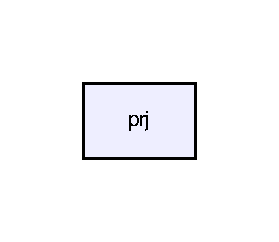
\includegraphics[width=134pt]{dir_00a2aeab00302c7b96c1830724320259_dep}
\end{center}
\end{figure}
\subsection*{\-Files}
\begin{DoxyCompactItemize}
\item 
file \hyperlink{generator_8cpp}{generator.\-cpp}
\item 
file \hyperlink{generator_8hh}{generator.\-hh}
\item 
file \hyperlink{graf_8cpp}{graf.\-cpp}
\item 
file \hyperlink{graf_8hh}{graf.\-hh}
\item 
file \hyperlink{komiwojazer_8cpp}{komiwojazer.\-cpp}
\item 
file \hyperlink{komiwojazer_8hh}{komiwojazer.\-hh}
\item 
file \hyperlink{main_8cpp}{main.\-cpp}
\item 
file \hyperlink{menu_8cpp}{menu.\-cpp}
\item 
file \hyperlink{menu_8hh}{menu.\-hh}
\item 
file \hyperlink{stoper_8hh}{stoper.\-hh}
\item 
file \hyperlink{wierzcholek_8cpp}{wierzcholek.\-cpp}
\item 
file \hyperlink{wierzcholek_8hh}{wierzcholek.\-hh}
\end{DoxyCompactItemize}

\chapter{\-Class \-Documentation}
\hypertarget{classczas}{\section{czas \-Class \-Reference}
\label{classczas}\index{czas@{czas}}
}


{\ttfamily \#include $<$stoper.\-hh$>$}

\subsection*{\-Public \-Member \-Functions}
\begin{DoxyCompactItemize}
\item 
void \hyperlink{classczas_a1e4c793526806f459e7f5c8c4a3ae29f}{start} ()
\begin{DoxyCompactList}\small\item\em start pomiaru zapisuje stan zegara \end{DoxyCompactList}\item 
void \hyperlink{classczas_a27f391e3c6bfb1f15f97c61bf403eb2d}{stop} ()
\begin{DoxyCompactList}\small\item\em koniec pomiaru zapisuje stan zegara \end{DoxyCompactList}\item 
void \hyperlink{classczas_a579654b3ae8126b00cf4d477f6d18d96}{wynik} ()
\begin{DoxyCompactList}\small\item\em zwraca wynik pomiaru \end{DoxyCompactList}\item 
void \hyperlink{classczas_a53e5d67a7dd77239f2ef6ae0866e0596}{zapisz} (fstream \&\hyperlink{classczas_a579654b3ae8126b00cf4d477f6d18d96}{wynik}, int rozmiar)
\begin{DoxyCompactList}\small\item\em zapisuje wynik do pliku \end{DoxyCompactList}\end{DoxyCompactItemize}
\subsection*{\-Public \-Attributes}
\begin{DoxyCompactItemize}
\item 
double \hyperlink{classczas_a1348fd4948270410b3087bb0318bd147}{time}
\end{DoxyCompactItemize}
\subsection*{\-Private \-Attributes}
\begin{DoxyCompactItemize}
\item 
clock\-\_\-t \hyperlink{classczas_a3e75d47bf9beee497b56997b0b7be45c}{poczatek}
\item 
clock\-\_\-t \hyperlink{classczas_a65324dff284c101f2594b0b05b30399e}{koniec}
\end{DoxyCompactItemize}


\subsection{\-Detailed \-Description}


\-Definition at line 19 of file stoper.\-hh.



\subsection{\-Member \-Function \-Documentation}
\hypertarget{classczas_a1e4c793526806f459e7f5c8c4a3ae29f}{\index{czas@{czas}!start@{start}}
\index{start@{start}!czas@{czas}}
\subsubsection[{start}]{\setlength{\rightskip}{0pt plus 5cm}void {\bf czas\-::start} (
\begin{DoxyParamCaption}
{}
\end{DoxyParamCaption}
)\hspace{0.3cm}{\ttfamily  \mbox{[}inline\mbox{]}}}}\label{classczas_a1e4c793526806f459e7f5c8c4a3ae29f}


\-Definition at line 31 of file stoper.\-hh.

\hypertarget{classczas_a27f391e3c6bfb1f15f97c61bf403eb2d}{\index{czas@{czas}!stop@{stop}}
\index{stop@{stop}!czas@{czas}}
\subsubsection[{stop}]{\setlength{\rightskip}{0pt plus 5cm}void {\bf czas\-::stop} (
\begin{DoxyParamCaption}
{}
\end{DoxyParamCaption}
)\hspace{0.3cm}{\ttfamily  \mbox{[}inline\mbox{]}}}}\label{classczas_a27f391e3c6bfb1f15f97c61bf403eb2d}


\-Definition at line 39 of file stoper.\-hh.

\hypertarget{classczas_a579654b3ae8126b00cf4d477f6d18d96}{\index{czas@{czas}!wynik@{wynik}}
\index{wynik@{wynik}!czas@{czas}}
\subsubsection[{wynik}]{\setlength{\rightskip}{0pt plus 5cm}void {\bf czas\-::wynik} (
\begin{DoxyParamCaption}
{}
\end{DoxyParamCaption}
)\hspace{0.3cm}{\ttfamily  \mbox{[}inline\mbox{]}}}}\label{classczas_a579654b3ae8126b00cf4d477f6d18d96}
\begin{DoxyReturn}{\-Returns}
zwraca czas dzialania 
\end{DoxyReturn}


\-Definition at line 47 of file stoper.\-hh.

\hypertarget{classczas_a53e5d67a7dd77239f2ef6ae0866e0596}{\index{czas@{czas}!zapisz@{zapisz}}
\index{zapisz@{zapisz}!czas@{czas}}
\subsubsection[{zapisz}]{\setlength{\rightskip}{0pt plus 5cm}void {\bf czas\-::zapisz} (
\begin{DoxyParamCaption}
\item[{fstream \&}]{wynik, }
\item[{int}]{rozmiar}
\end{DoxyParamCaption}
)\hspace{0.3cm}{\ttfamily  \mbox{[}inline\mbox{]}}}}\label{classczas_a53e5d67a7dd77239f2ef6ae0866e0596}

\begin{DoxyParams}{\-Parameters}
{\em wynik} & pomiaru \\
\hline
{\em rozmiar} & rozmiar problemu \\
\hline
\end{DoxyParams}


\-Definition at line 57 of file stoper.\-hh.



\subsection{\-Member \-Data \-Documentation}
\hypertarget{classczas_a65324dff284c101f2594b0b05b30399e}{\index{czas@{czas}!koniec@{koniec}}
\index{koniec@{koniec}!czas@{czas}}
\subsubsection[{koniec}]{\setlength{\rightskip}{0pt plus 5cm}clock\-\_\-t {\bf czas\-::koniec}\hspace{0.3cm}{\ttfamily  \mbox{[}private\mbox{]}}}}\label{classczas_a65324dff284c101f2594b0b05b30399e}


\-Definition at line 24 of file stoper.\-hh.

\hypertarget{classczas_a3e75d47bf9beee497b56997b0b7be45c}{\index{czas@{czas}!poczatek@{poczatek}}
\index{poczatek@{poczatek}!czas@{czas}}
\subsubsection[{poczatek}]{\setlength{\rightskip}{0pt plus 5cm}clock\-\_\-t {\bf czas\-::poczatek}\hspace{0.3cm}{\ttfamily  \mbox{[}private\mbox{]}}}}\label{classczas_a3e75d47bf9beee497b56997b0b7be45c}


\-Definition at line 24 of file stoper.\-hh.

\hypertarget{classczas_a1348fd4948270410b3087bb0318bd147}{\index{czas@{czas}!time@{time}}
\index{time@{time}!czas@{czas}}
\subsubsection[{time}]{\setlength{\rightskip}{0pt plus 5cm}double {\bf czas\-::time}}}\label{classczas_a1348fd4948270410b3087bb0318bd147}


\-Definition at line 26 of file stoper.\-hh.



\-The documentation for this class was generated from the following file\-:\begin{DoxyCompactItemize}
\item 
prj/\hyperlink{stoper_8hh}{stoper.\-hh}\end{DoxyCompactItemize}

\hypertarget{classdroga__komi}{\section{droga\-\_\-komi \-Class \-Reference}
\label{classdroga__komi}\index{droga\-\_\-komi@{droga\-\_\-komi}}
}


klasa modeluje pojecie drogi komiwojazera.  




{\ttfamily \#include $<$komiwojazer.\-hh$>$}



\-Collaboration diagram for droga\-\_\-komi\-:
\nopagebreak
\begin{figure}[H]
\begin{center}
\leavevmode
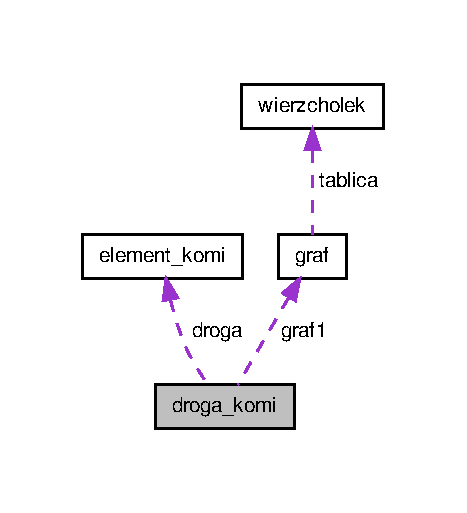
\includegraphics[width=224pt]{classdroga__komi__coll__graph}
\end{center}
\end{figure}
\subsection*{\-Public \-Member \-Functions}
\begin{DoxyCompactItemize}
\item 
\hyperlink{classdroga__komi_a4ac601fcf068b22d5cb6a4f0e9ae8386}{droga\-\_\-komi} (\hyperlink{classgraf}{graf} $\ast$obslugiwany)
\item 
\hyperlink{structpolaczenie}{polaczenie} \hyperlink{classdroga__komi_a1acfde1a8989daab4b6a03cbc660ea7e}{najblizszy} (int v, int start)
\begin{DoxyCompactList}\small\item\em funkcja wyznacza wierzcholek najblizej polozony \end{DoxyCompactList}\item 
void \hyperlink{classdroga__komi_a7d6a3684fd92f231b31597a24e3e6914}{trasa\-\_\-najblizsze} (int start)
\begin{DoxyCompactList}\small\item\em funckja tworzy petle hamiltona w zadanym grafie \end{DoxyCompactList}\item 
void \hyperlink{classdroga__komi_accef23783e2fc22179eee5aea746e0f4}{czytaj\-\_\-droge} (int v1)
\end{DoxyCompactItemize}
\subsection*{\-Private \-Attributes}
\begin{DoxyCompactItemize}
\item 
\hyperlink{classgraf}{graf} $\ast$ \hyperlink{classdroga__komi_a3bdab6c27afa54acc53a4a9f37b5745e}{graf1}
\item 
\hyperlink{structelement__komi}{element\-\_\-komi} $\ast$ \hyperlink{classdroga__komi_a4d4d9bdaaf335bb3ec6617acc60754ce}{droga}
\item 
int \hyperlink{classdroga__komi_a7f2bb9dfb6fdbdcdd67fa8e6bd53b0a6}{dlugosc}
\end{DoxyCompactItemize}


\subsection{\-Detailed \-Description}


\-Definition at line 28 of file komiwojazer.\-hh.



\subsection{\-Constructor \& \-Destructor \-Documentation}
\hypertarget{classdroga__komi_a4ac601fcf068b22d5cb6a4f0e9ae8386}{\index{droga\-\_\-komi@{droga\-\_\-komi}!droga\-\_\-komi@{droga\-\_\-komi}}
\index{droga\-\_\-komi@{droga\-\_\-komi}!droga_komi@{droga\-\_\-komi}}
\subsubsection[{droga\-\_\-komi}]{\setlength{\rightskip}{0pt plus 5cm}{\bf droga\-\_\-komi\-::droga\-\_\-komi} (
\begin{DoxyParamCaption}
\item[{{\bf graf} $\ast$}]{obslugiwany}
\end{DoxyParamCaption}
)}}\label{classdroga__komi_a4ac601fcf068b22d5cb6a4f0e9ae8386}


\-Definition at line 9 of file komiwojazer.\-cpp.



\subsection{\-Member \-Function \-Documentation}
\hypertarget{classdroga__komi_accef23783e2fc22179eee5aea746e0f4}{\index{droga\-\_\-komi@{droga\-\_\-komi}!czytaj\-\_\-droge@{czytaj\-\_\-droge}}
\index{czytaj\-\_\-droge@{czytaj\-\_\-droge}!droga_komi@{droga\-\_\-komi}}
\subsubsection[{czytaj\-\_\-droge}]{\setlength{\rightskip}{0pt plus 5cm}void {\bf droga\-\_\-komi\-::czytaj\-\_\-droge} (
\begin{DoxyParamCaption}
\item[{int}]{v1}
\end{DoxyParamCaption}
)}}\label{classdroga__komi_accef23783e2fc22179eee5aea746e0f4}


\-Definition at line 64 of file komiwojazer.\-cpp.



\-Here is the caller graph for this function\-:
\nopagebreak
\begin{figure}[H]
\begin{center}
\leavevmode
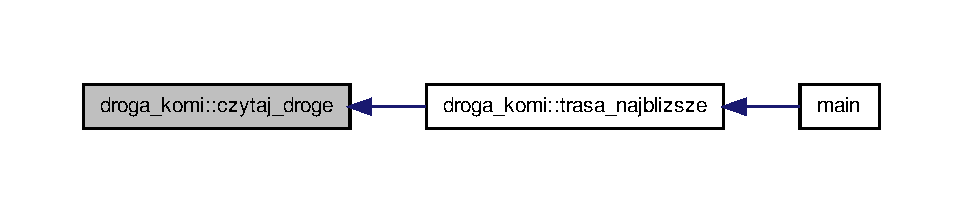
\includegraphics[width=350pt]{classdroga__komi_accef23783e2fc22179eee5aea746e0f4_icgraph}
\end{center}
\end{figure}


\hypertarget{classdroga__komi_a1acfde1a8989daab4b6a03cbc660ea7e}{\index{droga\-\_\-komi@{droga\-\_\-komi}!najblizszy@{najblizszy}}
\index{najblizszy@{najblizszy}!droga_komi@{droga\-\_\-komi}}
\subsubsection[{najblizszy}]{\setlength{\rightskip}{0pt plus 5cm}{\bf polaczenie} {\bf droga\-\_\-komi\-::najblizszy} (
\begin{DoxyParamCaption}
\item[{int}]{v, }
\item[{int}]{start}
\end{DoxyParamCaption}
)}}\label{classdroga__komi_a1acfde1a8989daab4b6a03cbc660ea7e}

\begin{DoxyParams}{\-Parameters}
{\em start} & \\
\hline
\end{DoxyParams}
lista polaczen wierzcholka 

\-Definition at line 43 of file komiwojazer.\-cpp.



\-Here is the call graph for this function\-:
\nopagebreak
\begin{figure}[H]
\begin{center}
\leavevmode
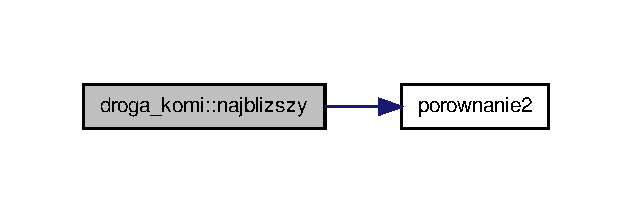
\includegraphics[width=304pt]{classdroga__komi_a1acfde1a8989daab4b6a03cbc660ea7e_cgraph}
\end{center}
\end{figure}




\-Here is the caller graph for this function\-:
\nopagebreak
\begin{figure}[H]
\begin{center}
\leavevmode
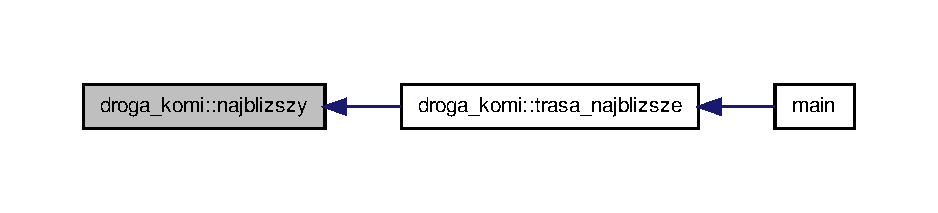
\includegraphics[width=350pt]{classdroga__komi_a1acfde1a8989daab4b6a03cbc660ea7e_icgraph}
\end{center}
\end{figure}


\hypertarget{classdroga__komi_a7d6a3684fd92f231b31597a24e3e6914}{\index{droga\-\_\-komi@{droga\-\_\-komi}!trasa\-\_\-najblizsze@{trasa\-\_\-najblizsze}}
\index{trasa\-\_\-najblizsze@{trasa\-\_\-najblizsze}!droga_komi@{droga\-\_\-komi}}
\subsubsection[{trasa\-\_\-najblizsze}]{\setlength{\rightskip}{0pt plus 5cm}void {\bf droga\-\_\-komi\-::trasa\-\_\-najblizsze} (
\begin{DoxyParamCaption}
\item[{int}]{start}
\end{DoxyParamCaption}
)}}\label{classdroga__komi_a7d6a3684fd92f231b31597a24e3e6914}
alfgorytm laczy wierzcholek z nastepnym najblizej polaczonym az wszystkie wierzcholki zostana polaczone w petle. 
\begin{DoxyParams}{\-Parameters}
{\em obslugiwany} & \\
\hline
\end{DoxyParams}


\-Definition at line 22 of file komiwojazer.\-cpp.



\-Here is the call graph for this function\-:
\nopagebreak
\begin{figure}[H]
\begin{center}
\leavevmode
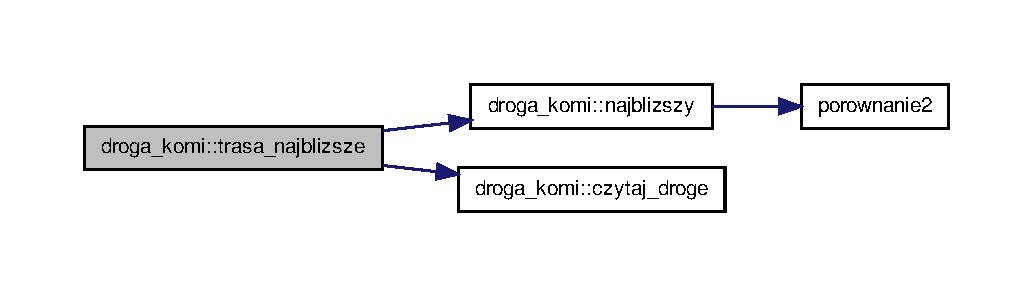
\includegraphics[width=350pt]{classdroga__komi_a7d6a3684fd92f231b31597a24e3e6914_cgraph}
\end{center}
\end{figure}




\-Here is the caller graph for this function\-:
\nopagebreak
\begin{figure}[H]
\begin{center}
\leavevmode
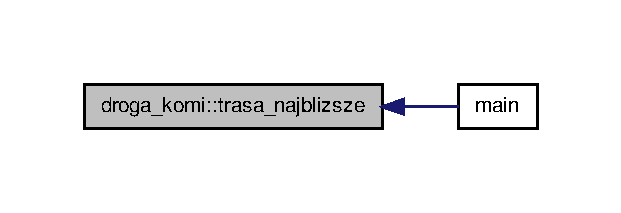
\includegraphics[width=298pt]{classdroga__komi_a7d6a3684fd92f231b31597a24e3e6914_icgraph}
\end{center}
\end{figure}




\subsection{\-Member \-Data \-Documentation}
\hypertarget{classdroga__komi_a7f2bb9dfb6fdbdcdd67fa8e6bd53b0a6}{\index{droga\-\_\-komi@{droga\-\_\-komi}!dlugosc@{dlugosc}}
\index{dlugosc@{dlugosc}!droga_komi@{droga\-\_\-komi}}
\subsubsection[{dlugosc}]{\setlength{\rightskip}{0pt plus 5cm}int {\bf droga\-\_\-komi\-::dlugosc}\hspace{0.3cm}{\ttfamily  \mbox{[}private\mbox{]}}}}\label{classdroga__komi_a7f2bb9dfb6fdbdcdd67fa8e6bd53b0a6}


\-Definition at line 32 of file komiwojazer.\-hh.

\hypertarget{classdroga__komi_a4d4d9bdaaf335bb3ec6617acc60754ce}{\index{droga\-\_\-komi@{droga\-\_\-komi}!droga@{droga}}
\index{droga@{droga}!droga_komi@{droga\-\_\-komi}}
\subsubsection[{droga}]{\setlength{\rightskip}{0pt plus 5cm}{\bf element\-\_\-komi}$\ast$ {\bf droga\-\_\-komi\-::droga}\hspace{0.3cm}{\ttfamily  \mbox{[}private\mbox{]}}}}\label{classdroga__komi_a4d4d9bdaaf335bb3ec6617acc60754ce}


\-Definition at line 31 of file komiwojazer.\-hh.

\hypertarget{classdroga__komi_a3bdab6c27afa54acc53a4a9f37b5745e}{\index{droga\-\_\-komi@{droga\-\_\-komi}!graf1@{graf1}}
\index{graf1@{graf1}!droga_komi@{droga\-\_\-komi}}
\subsubsection[{graf1}]{\setlength{\rightskip}{0pt plus 5cm}{\bf graf}$\ast$ {\bf droga\-\_\-komi\-::graf1}\hspace{0.3cm}{\ttfamily  \mbox{[}private\mbox{]}}}}\label{classdroga__komi_a3bdab6c27afa54acc53a4a9f37b5745e}


\-Definition at line 30 of file komiwojazer.\-hh.



\-The documentation for this class was generated from the following files\-:\begin{DoxyCompactItemize}
\item 
prj/\hyperlink{komiwojazer_8hh}{komiwojazer.\-hh}\item 
prj/\hyperlink{komiwojazer_8cpp}{komiwojazer.\-cpp}\end{DoxyCompactItemize}

\hypertarget{structelement__a}{\section{element\-\_\-a \-Struct \-Reference}
\label{structelement__a}\index{element\-\_\-a@{element\-\_\-a}}
}


{\ttfamily \#include $<$wierzcholek.\-hh$>$}

\subsection*{\-Public \-Member \-Functions}
\begin{DoxyCompactItemize}
\item 
\hyperlink{structelement__a_a75d6e0125b7bd95c6d2012332cdf3957}{element\-\_\-a} ()
\end{DoxyCompactItemize}
\subsection*{\-Public \-Attributes}
\begin{DoxyCompactItemize}
\item 
int \hyperlink{structelement__a_acebbe0c4962a9b7f11702c041474bdfc}{wierzcholek}
\item 
int \hyperlink{structelement__a_a0c44e77b4e694ff0f7e2a5ec75a78f48}{waga}
\item 
int \hyperlink{structelement__a_a4e6b23a45c539eea4ab51d74aeef11e2}{poprzedni}
\item 
int \hyperlink{structelement__a_a1be911aa9cf4faf7105ae58ec04d4bd7}{stan}
\end{DoxyCompactItemize}


\subsection{\-Detailed \-Description}


\-Definition at line 103 of file wierzcholek.\-hh.



\subsection{\-Constructor \& \-Destructor \-Documentation}
\hypertarget{structelement__a_a75d6e0125b7bd95c6d2012332cdf3957}{\index{element\-\_\-a@{element\-\_\-a}!element\-\_\-a@{element\-\_\-a}}
\index{element\-\_\-a@{element\-\_\-a}!element_a@{element\-\_\-a}}
\subsubsection[{element\-\_\-a}]{\setlength{\rightskip}{0pt plus 5cm}{\bf element\-\_\-a\-::element\-\_\-a} (
\begin{DoxyParamCaption}
{}
\end{DoxyParamCaption}
)\hspace{0.3cm}{\ttfamily  \mbox{[}inline\mbox{]}}}}\label{structelement__a_a75d6e0125b7bd95c6d2012332cdf3957}


\-Definition at line 109 of file wierzcholek.\-hh.



\subsection{\-Member \-Data \-Documentation}
\hypertarget{structelement__a_a4e6b23a45c539eea4ab51d74aeef11e2}{\index{element\-\_\-a@{element\-\_\-a}!poprzedni@{poprzedni}}
\index{poprzedni@{poprzedni}!element_a@{element\-\_\-a}}
\subsubsection[{poprzedni}]{\setlength{\rightskip}{0pt plus 5cm}int {\bf element\-\_\-a\-::poprzedni}}}\label{structelement__a_a4e6b23a45c539eea4ab51d74aeef11e2}


\-Definition at line 107 of file wierzcholek.\-hh.

\hypertarget{structelement__a_a1be911aa9cf4faf7105ae58ec04d4bd7}{\index{element\-\_\-a@{element\-\_\-a}!stan@{stan}}
\index{stan@{stan}!element_a@{element\-\_\-a}}
\subsubsection[{stan}]{\setlength{\rightskip}{0pt plus 5cm}int {\bf element\-\_\-a\-::stan}}}\label{structelement__a_a1be911aa9cf4faf7105ae58ec04d4bd7}


\-Definition at line 108 of file wierzcholek.\-hh.

\hypertarget{structelement__a_a0c44e77b4e694ff0f7e2a5ec75a78f48}{\index{element\-\_\-a@{element\-\_\-a}!waga@{waga}}
\index{waga@{waga}!element_a@{element\-\_\-a}}
\subsubsection[{waga}]{\setlength{\rightskip}{0pt plus 5cm}int {\bf element\-\_\-a\-::waga}}}\label{structelement__a_a0c44e77b4e694ff0f7e2a5ec75a78f48}


\-Definition at line 106 of file wierzcholek.\-hh.

\hypertarget{structelement__a_acebbe0c4962a9b7f11702c041474bdfc}{\index{element\-\_\-a@{element\-\_\-a}!wierzcholek@{wierzcholek}}
\index{wierzcholek@{wierzcholek}!element_a@{element\-\_\-a}}
\subsubsection[{wierzcholek}]{\setlength{\rightskip}{0pt plus 5cm}int {\bf element\-\_\-a\-::wierzcholek}}}\label{structelement__a_acebbe0c4962a9b7f11702c041474bdfc}


\-Definition at line 105 of file wierzcholek.\-hh.



\-The documentation for this struct was generated from the following file\-:\begin{DoxyCompactItemize}
\item 
prj/\hyperlink{wierzcholek_8hh}{wierzcholek.\-hh}\end{DoxyCompactItemize}

\hypertarget{structelement__bfs}{\section{element\-\_\-bfs \-Struct \-Reference}
\label{structelement__bfs}\index{element\-\_\-bfs@{element\-\_\-bfs}}
}


struktura definiuje element drzewa przechodzenie w szerz  




{\ttfamily \#include $<$wierzcholek.\-hh$>$}

\subsection*{\-Public \-Member \-Functions}
\begin{DoxyCompactItemize}
\item 
\hyperlink{structelement__bfs_a9c764ce268e74260e6634ea98ed13781}{element\-\_\-bfs} ()
\end{DoxyCompactItemize}
\subsection*{\-Public \-Attributes}
\begin{DoxyCompactItemize}
\item 
int \hyperlink{structelement__bfs_aa654df64808f513f41d0349571e4b90e}{stan}
\item 
int \hyperlink{structelement__bfs_a91fcdfed5d5dc2bce6ca9bb4414df196}{odleglosc}
\item 
int \hyperlink{structelement__bfs_a94b882f6922be485d6942f71c29e581d}{poprzedni}
\end{DoxyCompactItemize}
\subsection*{\-Friends}
\begin{DoxyCompactItemize}
\item 
ostream \& \hyperlink{structelement__bfs_a8b076b347dc8398fd7e704d74299eb3a}{operator$<$$<$} (ostream \&wyjscie, \hyperlink{structelement__bfs}{element\-\_\-bfs} \&dane)
\end{DoxyCompactItemize}


\subsection{\-Detailed \-Description}


\-Definition at line 64 of file wierzcholek.\-hh.



\subsection{\-Constructor \& \-Destructor \-Documentation}
\hypertarget{structelement__bfs_a9c764ce268e74260e6634ea98ed13781}{\index{element\-\_\-bfs@{element\-\_\-bfs}!element\-\_\-bfs@{element\-\_\-bfs}}
\index{element\-\_\-bfs@{element\-\_\-bfs}!element_bfs@{element\-\_\-bfs}}
\subsubsection[{element\-\_\-bfs}]{\setlength{\rightskip}{0pt plus 5cm}{\bf element\-\_\-bfs\-::element\-\_\-bfs} (
\begin{DoxyParamCaption}
{}
\end{DoxyParamCaption}
)\hspace{0.3cm}{\ttfamily  \mbox{[}inline\mbox{]}}}}\label{structelement__bfs_a9c764ce268e74260e6634ea98ed13781}


\-Definition at line 69 of file wierzcholek.\-hh.



\subsection{\-Friends \-And \-Related \-Function \-Documentation}
\hypertarget{structelement__bfs_a8b076b347dc8398fd7e704d74299eb3a}{\index{element\-\_\-bfs@{element\-\_\-bfs}!operator$<$$<$@{operator$<$$<$}}
\index{operator$<$$<$@{operator$<$$<$}!element_bfs@{element\-\_\-bfs}}
\subsubsection[{operator$<$$<$}]{\setlength{\rightskip}{0pt plus 5cm}ostream\& operator$<$$<$ (
\begin{DoxyParamCaption}
\item[{ostream \&}]{wyjscie, }
\item[{{\bf element\-\_\-bfs} \&}]{dane}
\end{DoxyParamCaption}
)\hspace{0.3cm}{\ttfamily  \mbox{[}friend\mbox{]}}}}\label{structelement__bfs_a8b076b347dc8398fd7e704d74299eb3a}


\-Definition at line 71 of file wierzcholek.\-hh.



\subsection{\-Member \-Data \-Documentation}
\hypertarget{structelement__bfs_a91fcdfed5d5dc2bce6ca9bb4414df196}{\index{element\-\_\-bfs@{element\-\_\-bfs}!odleglosc@{odleglosc}}
\index{odleglosc@{odleglosc}!element_bfs@{element\-\_\-bfs}}
\subsubsection[{odleglosc}]{\setlength{\rightskip}{0pt plus 5cm}int {\bf element\-\_\-bfs\-::odleglosc}}}\label{structelement__bfs_a91fcdfed5d5dc2bce6ca9bb4414df196}


\-Definition at line 67 of file wierzcholek.\-hh.

\hypertarget{structelement__bfs_a94b882f6922be485d6942f71c29e581d}{\index{element\-\_\-bfs@{element\-\_\-bfs}!poprzedni@{poprzedni}}
\index{poprzedni@{poprzedni}!element_bfs@{element\-\_\-bfs}}
\subsubsection[{poprzedni}]{\setlength{\rightskip}{0pt plus 5cm}int {\bf element\-\_\-bfs\-::poprzedni}}}\label{structelement__bfs_a94b882f6922be485d6942f71c29e581d}


\-Definition at line 68 of file wierzcholek.\-hh.

\hypertarget{structelement__bfs_aa654df64808f513f41d0349571e4b90e}{\index{element\-\_\-bfs@{element\-\_\-bfs}!stan@{stan}}
\index{stan@{stan}!element_bfs@{element\-\_\-bfs}}
\subsubsection[{stan}]{\setlength{\rightskip}{0pt plus 5cm}int {\bf element\-\_\-bfs\-::stan}}}\label{structelement__bfs_aa654df64808f513f41d0349571e4b90e}


\-Definition at line 66 of file wierzcholek.\-hh.



\-The documentation for this struct was generated from the following file\-:\begin{DoxyCompactItemize}
\item 
prj/\hyperlink{wierzcholek_8hh}{wierzcholek.\-hh}\end{DoxyCompactItemize}

\hypertarget{structelement__dfs}{\section{element\-\_\-dfs \-Struct \-Reference}
\label{structelement__dfs}\index{element\-\_\-dfs@{element\-\_\-dfs}}
}


element drzewa przejscia dla przeszukiwania w głąb;  




{\ttfamily \#include $<$wierzcholek.\-hh$>$}

\subsection*{\-Public \-Member \-Functions}
\begin{DoxyCompactItemize}
\item 
\hyperlink{structelement__dfs_a7a70ed0a00bcaafd111e9b07a135bbe4}{element\-\_\-dfs} ()
\end{DoxyCompactItemize}
\subsection*{\-Public \-Attributes}
\begin{DoxyCompactItemize}
\item 
int \hyperlink{structelement__dfs_a48b8257c62eb0f4c52e10bf2c06fffda}{stan}
\item 
int \hyperlink{structelement__dfs_af3205a446fe8c834532d3b5de81deefa}{poprzedni}
\item 
int \hyperlink{structelement__dfs_ae2d3c82805dc8b9b24a7dc1511c283dd}{d}
\begin{DoxyCompactList}\small\item\em czas wejscia do wierzcholka \end{DoxyCompactList}\item 
int \hyperlink{structelement__dfs_a9a75ad927680701485941a4e42b36290}{f}
\begin{DoxyCompactList}\small\item\em czas wyjscia z wierzcholka \end{DoxyCompactList}\end{DoxyCompactItemize}
\subsection*{\-Friends}
\begin{DoxyCompactItemize}
\item 
ostream \& \hyperlink{structelement__dfs_abb6d36003fb4e11d878e4bd1d794469b}{operator$<$$<$} (ostream \&wyjscie, \hyperlink{structelement__dfs}{element\-\_\-dfs} \&dane)
\end{DoxyCompactItemize}


\subsection{\-Detailed \-Description}


\-Definition at line 68 of file wierzcholek.\-hh.



\subsection{\-Constructor \& \-Destructor \-Documentation}
\hypertarget{structelement__dfs_a7a70ed0a00bcaafd111e9b07a135bbe4}{\index{element\-\_\-dfs@{element\-\_\-dfs}!element\-\_\-dfs@{element\-\_\-dfs}}
\index{element\-\_\-dfs@{element\-\_\-dfs}!element_dfs@{element\-\_\-dfs}}
\subsubsection[{element\-\_\-dfs}]{\setlength{\rightskip}{0pt plus 5cm}{\bf element\-\_\-dfs\-::element\-\_\-dfs} (
\begin{DoxyParamCaption}
{}
\end{DoxyParamCaption}
)\hspace{0.3cm}{\ttfamily  \mbox{[}inline\mbox{]}}}}\label{structelement__dfs_a7a70ed0a00bcaafd111e9b07a135bbe4}


\-Definition at line 76 of file wierzcholek.\-hh.



\subsection{\-Friends \-And \-Related \-Function \-Documentation}
\hypertarget{structelement__dfs_abb6d36003fb4e11d878e4bd1d794469b}{\index{element\-\_\-dfs@{element\-\_\-dfs}!operator$<$$<$@{operator$<$$<$}}
\index{operator$<$$<$@{operator$<$$<$}!element_dfs@{element\-\_\-dfs}}
\subsubsection[{operator$<$$<$}]{\setlength{\rightskip}{0pt plus 5cm}ostream\& operator$<$$<$ (
\begin{DoxyParamCaption}
\item[{ostream \&}]{wyjscie, }
\item[{{\bf element\-\_\-dfs} \&}]{dane}
\end{DoxyParamCaption}
)\hspace{0.3cm}{\ttfamily  \mbox{[}friend\mbox{]}}}}\label{structelement__dfs_abb6d36003fb4e11d878e4bd1d794469b}


\-Definition at line 78 of file wierzcholek.\-hh.



\subsection{\-Member \-Data \-Documentation}
\hypertarget{structelement__dfs_ae2d3c82805dc8b9b24a7dc1511c283dd}{\index{element\-\_\-dfs@{element\-\_\-dfs}!d@{d}}
\index{d@{d}!element_dfs@{element\-\_\-dfs}}
\subsubsection[{d}]{\setlength{\rightskip}{0pt plus 5cm}int {\bf element\-\_\-dfs\-::d}}}\label{structelement__dfs_ae2d3c82805dc8b9b24a7dc1511c283dd}


\-Definition at line 73 of file wierzcholek.\-hh.

\hypertarget{structelement__dfs_a9a75ad927680701485941a4e42b36290}{\index{element\-\_\-dfs@{element\-\_\-dfs}!f@{f}}
\index{f@{f}!element_dfs@{element\-\_\-dfs}}
\subsubsection[{f}]{\setlength{\rightskip}{0pt plus 5cm}int {\bf element\-\_\-dfs\-::f}}}\label{structelement__dfs_a9a75ad927680701485941a4e42b36290}


\-Definition at line 75 of file wierzcholek.\-hh.

\hypertarget{structelement__dfs_af3205a446fe8c834532d3b5de81deefa}{\index{element\-\_\-dfs@{element\-\_\-dfs}!poprzedni@{poprzedni}}
\index{poprzedni@{poprzedni}!element_dfs@{element\-\_\-dfs}}
\subsubsection[{poprzedni}]{\setlength{\rightskip}{0pt plus 5cm}int {\bf element\-\_\-dfs\-::poprzedni}}}\label{structelement__dfs_af3205a446fe8c834532d3b5de81deefa}


\-Definition at line 71 of file wierzcholek.\-hh.

\hypertarget{structelement__dfs_a48b8257c62eb0f4c52e10bf2c06fffda}{\index{element\-\_\-dfs@{element\-\_\-dfs}!stan@{stan}}
\index{stan@{stan}!element_dfs@{element\-\_\-dfs}}
\subsubsection[{stan}]{\setlength{\rightskip}{0pt plus 5cm}int {\bf element\-\_\-dfs\-::stan}}}\label{structelement__dfs_a48b8257c62eb0f4c52e10bf2c06fffda}


\-Definition at line 70 of file wierzcholek.\-hh.



\-The documentation for this struct was generated from the following file\-:\begin{DoxyCompactItemize}
\item 
prj/\hyperlink{wierzcholek_8hh}{wierzcholek.\-hh}\end{DoxyCompactItemize}

\hypertarget{structelement__komi}{\section{element\-\_\-komi \-Struct \-Reference}
\label{structelement__komi}\index{element\-\_\-komi@{element\-\_\-komi}}
}


klasa modeluje element drogi komiwojazera  




{\ttfamily \#include $<$komiwojazer.\-hh$>$}

\subsection*{\-Public \-Member \-Functions}
\begin{DoxyCompactItemize}
\item 
\hyperlink{structelement__komi_a9ff04abc2364d58aedde507d71cfb88d}{element\-\_\-komi} ()
\end{DoxyCompactItemize}
\subsection*{\-Public \-Attributes}
\begin{DoxyCompactItemize}
\item 
bool \hyperlink{structelement__komi_a85030e1988969c8bd43cafbb006a8bff}{stan}
\item 
int \hyperlink{structelement__komi_a30a791cf42a38534bf589661aaf680d5}{nastepny}
\item 
int \hyperlink{structelement__komi_a6d353ba2bf60e3e6161af6957edf2be0}{waga}
\end{DoxyCompactItemize}


\subsection{\-Detailed \-Description}


\-Definition at line 16 of file komiwojazer.\-hh.



\subsection{\-Constructor \& \-Destructor \-Documentation}
\hypertarget{structelement__komi_a9ff04abc2364d58aedde507d71cfb88d}{\index{element\-\_\-komi@{element\-\_\-komi}!element\-\_\-komi@{element\-\_\-komi}}
\index{element\-\_\-komi@{element\-\_\-komi}!element_komi@{element\-\_\-komi}}
\subsubsection[{element\-\_\-komi}]{\setlength{\rightskip}{0pt plus 5cm}{\bf element\-\_\-komi\-::element\-\_\-komi} (
\begin{DoxyParamCaption}
{}
\end{DoxyParamCaption}
)\hspace{0.3cm}{\ttfamily  \mbox{[}inline\mbox{]}}}}\label{structelement__komi_a9ff04abc2364d58aedde507d71cfb88d}


\-Definition at line 21 of file komiwojazer.\-hh.



\subsection{\-Member \-Data \-Documentation}
\hypertarget{structelement__komi_a30a791cf42a38534bf589661aaf680d5}{\index{element\-\_\-komi@{element\-\_\-komi}!nastepny@{nastepny}}
\index{nastepny@{nastepny}!element_komi@{element\-\_\-komi}}
\subsubsection[{nastepny}]{\setlength{\rightskip}{0pt plus 5cm}int {\bf element\-\_\-komi\-::nastepny}}}\label{structelement__komi_a30a791cf42a38534bf589661aaf680d5}


\-Definition at line 19 of file komiwojazer.\-hh.

\hypertarget{structelement__komi_a85030e1988969c8bd43cafbb006a8bff}{\index{element\-\_\-komi@{element\-\_\-komi}!stan@{stan}}
\index{stan@{stan}!element_komi@{element\-\_\-komi}}
\subsubsection[{stan}]{\setlength{\rightskip}{0pt plus 5cm}bool {\bf element\-\_\-komi\-::stan}}}\label{structelement__komi_a85030e1988969c8bd43cafbb006a8bff}


\-Definition at line 18 of file komiwojazer.\-hh.

\hypertarget{structelement__komi_a6d353ba2bf60e3e6161af6957edf2be0}{\index{element\-\_\-komi@{element\-\_\-komi}!waga@{waga}}
\index{waga@{waga}!element_komi@{element\-\_\-komi}}
\subsubsection[{waga}]{\setlength{\rightskip}{0pt plus 5cm}int {\bf element\-\_\-komi\-::waga}}}\label{structelement__komi_a6d353ba2bf60e3e6161af6957edf2be0}


\-Definition at line 20 of file komiwojazer.\-hh.



\-The documentation for this struct was generated from the following file\-:\begin{DoxyCompactItemize}
\item 
prj/\hyperlink{komiwojazer_8hh}{komiwojazer.\-hh}\end{DoxyCompactItemize}

\hypertarget{classgraf}{\section{graf \-Class \-Reference}
\label{classgraf}\index{graf@{graf}}
}


klasa modeluje graf.  




{\ttfamily \#include $<$graf.\-hh$>$}



\-Collaboration diagram for graf\-:
\nopagebreak
\begin{figure}[H]
\begin{center}
\leavevmode
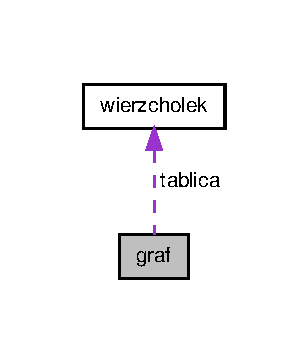
\includegraphics[width=236pt]{classgraf__coll__graph}
\end{center}
\end{figure}
\subsection*{\-Public \-Member \-Functions}
\begin{DoxyCompactItemize}
\item 
\hyperlink{classgraf_a66fe29b772c7e3085b161a31682ef093}{graf} (int il)
\begin{DoxyCompactList}\small\item\em konstruktor klasy graf \end{DoxyCompactList}\item 
\hyperlink{classgraf_a9aefd40799975c316a17bd67021e05f2}{$\sim$graf} ()
\begin{DoxyCompactList}\small\item\em destruktor grafu \end{DoxyCompactList}\item 
int \hyperlink{classgraf_aa045d28e07e38ca32adf1b353077f877}{wrozmiar} ()
\begin{DoxyCompactList}\small\item\em funkcja zwraca rozmiar grafu \end{DoxyCompactList}\item 
void \hyperlink{classgraf_a97c2722a11d3a7f90c82bc9b1cd56ef6}{wyswietl\-\_\-dfs} ()
\begin{DoxyCompactList}\small\item\em funkcja wyswietla \char`\"{}las drzew przejsc\char`\"{} \end{DoxyCompactList}\item 
void \hyperlink{classgraf_a6a50b0bfb5fc3cfc7a443014170b9565}{dodaj\-\_\-wierzcholek} (\hyperlink{classwierzcholek}{wierzcholek} nowy)
\begin{DoxyCompactList}\small\item\em funkcja sluzy do dodawania wierzcholkow \end{DoxyCompactList}\item 
void \hyperlink{classgraf_afaa55f5a9aef1f30a2b3be97b59a476b}{dodaj\-\_\-wierzcholek} ()
\begin{DoxyCompactList}\small\item\em funkcja dodaje wierzcholek \end{DoxyCompactList}\item 
void \hyperlink{classgraf_aa70de90b152f2cf47dac635793bcc5c4}{dodaj\-\_\-polaczenie} (int v1, int v2)
\begin{DoxyCompactList}\small\item\em funkcja dodaje polaczenie miedzy zadanymi wierzcholkami \end{DoxyCompactList}\item 
void \hyperlink{classgraf_ac7e01e940f136f4020e4da816c2fb1b4}{usun\-\_\-polaczenie} (int v1, int v2)
\begin{DoxyCompactList}\small\item\em funkcja usuwa polaczenie miedzy zadanymi wierzcholkami \end{DoxyCompactList}\item 
void \hyperlink{classgraf_a369202eb63332e9faad779591c862ece}{usun\-\_\-wierzcholek} (int numer)
\begin{DoxyCompactList}\small\item\em funkcja usuwa wierzcholek o zadanym kluczu \end{DoxyCompactList}\item 
void \hyperlink{classgraf_a8dd83fa1722d917a143b2da9245b5db9}{wyswietl\-\_\-sasiadow} (int numer)
\begin{DoxyCompactList}\small\item\em funkcja wyswietla sasiadow wierzcholka \end{DoxyCompactList}\item 
bool \hyperlink{classgraf_ae1ebd85c7cb288174a5dccc5fd90634e}{sprawdz\-\_\-polaczenie} (int v1, int v2)
\begin{DoxyCompactList}\small\item\em funkcja sprawdza czy mieszy podanymi wierzchokami istnieje polaczenie \end{DoxyCompactList}\item 
\hyperlink{structelement__bfs}{element\-\_\-bfs} $\ast$ \hyperlink{classgraf_a5b67e5e829440e984782b232188a5f57}{przejdz\-\_\-bfs} (int v1)
\begin{DoxyCompactList}\small\item\em implementacja algorytmu przechodzenie wszerz grafu \end{DoxyCompactList}\item 
void $\ast$ \hyperlink{classgraf_a4947702a6d93feb805b1e11e14ec1e13}{przejdz\-\_\-dfs} ()
\begin{DoxyCompactList}\small\item\em funkcja wywyołuje przejscie wglab drzewa dla kazdego nie odwiedzonego wierzcholka  to stworzenie paru drzew przejscia \end{DoxyCompactList}\item 
void \hyperlink{classgraf_a84527840c48cc131f9ef2ca493550ea0}{dfs\-\_\-visit} (int v1)
\begin{DoxyCompactList}\small\item\em funkcja przechodzi w głąb graf tworzac drzewo przejscia \end{DoxyCompactList}\end{DoxyCompactItemize}
\subsection*{\-Private \-Attributes}
\begin{DoxyCompactItemize}
\item 
\hyperlink{classwierzcholek}{wierzcholek} $\ast$ \hyperlink{classgraf_a028d547c797438718da6241a28b32db5}{tablica}
\item 
int \hyperlink{classgraf_a596da8a77b680d7ec408b1253c2c43c3}{rozmiar}
\item 
int \hyperlink{classgraf_ad9204c0bbc75a2bef4a43200672f9694}{ilosc}
\item 
int \hyperlink{classgraf_a9202cb6ab351f5bbdbb79de440ab1fb5}{time}
\item 
\hyperlink{structelement__dfs}{element\-\_\-dfs} $\ast$ \hyperlink{classgraf_a325616745236599f83bffb58d61b0fa9}{tablica\-\_\-dfs}
\end{DoxyCompactItemize}
\subsection*{\-Friends}
\begin{DoxyCompactItemize}
\item 
class \hyperlink{classgraf_af2b2242aa53a3230ae67c7b57d7d9d11}{bfs}
\item 
ostream \& \hyperlink{classgraf_aaf525f8cdadbe40d9ad7c39f79fd8a2c}{operator$<$$<$} (ostream \&wyjscie, \hyperlink{classgraf}{graf} \&dane)
\begin{DoxyCompactList}\small\item\em przeladowanie operatora wyjscia \end{DoxyCompactList}\end{DoxyCompactItemize}


\subsection{\-Detailed \-Description}
w klasie przechowywana jest tablica wierzcholkow oraz informacje mozliwej ilosci wierzcholkow i ilosci wierzcholkow wykorzystanych 

\-Definition at line 27 of file graf.\-hh.



\subsection{\-Constructor \& \-Destructor \-Documentation}
\hypertarget{classgraf_a66fe29b772c7e3085b161a31682ef093}{\index{graf@{graf}!graf@{graf}}
\index{graf@{graf}!graf@{graf}}
\subsubsection[{graf}]{\setlength{\rightskip}{0pt plus 5cm}{\bf graf\-::graf} (
\begin{DoxyParamCaption}
\item[{int}]{il}
\end{DoxyParamCaption}
)}}\label{classgraf_a66fe29b772c7e3085b161a31682ef093}

\begin{DoxyParams}{\-Parameters}
{\em il} & wielkosc tworzonego grafu \\
\hline
\end{DoxyParams}


\-Definition at line 30 of file graf.\-cpp.

\hypertarget{classgraf_a9aefd40799975c316a17bd67021e05f2}{\index{graf@{graf}!$\sim$graf@{$\sim$graf}}
\index{$\sim$graf@{$\sim$graf}!graf@{graf}}
\subsubsection[{$\sim$graf}]{\setlength{\rightskip}{0pt plus 5cm}{\bf graf\-::$\sim$graf} (
\begin{DoxyParamCaption}
{}
\end{DoxyParamCaption}
)}}\label{classgraf_a9aefd40799975c316a17bd67021e05f2}


\-Definition at line 42 of file graf.\-cpp.



\subsection{\-Member \-Function \-Documentation}
\hypertarget{classgraf_a84527840c48cc131f9ef2ca493550ea0}{\index{graf@{graf}!dfs\-\_\-visit@{dfs\-\_\-visit}}
\index{dfs\-\_\-visit@{dfs\-\_\-visit}!graf@{graf}}
\subsubsection[{dfs\-\_\-visit}]{\setlength{\rightskip}{0pt plus 5cm}void {\bf graf\-::dfs\-\_\-visit} (
\begin{DoxyParamCaption}
\item[{int}]{v1}
\end{DoxyParamCaption}
)}}\label{classgraf_a84527840c48cc131f9ef2ca493550ea0}
funkcja zaisuje czas odwiedzin oraz czas wyjscia z wierzcholka 
\begin{DoxyParams}{\-Parameters}
{\em v1} & \\
\hline
\end{DoxyParams}


\-Definition at line 285 of file graf.\-cpp.



\-Here is the caller graph for this function\-:
\nopagebreak
\begin{figure}[H]
\begin{center}
\leavevmode
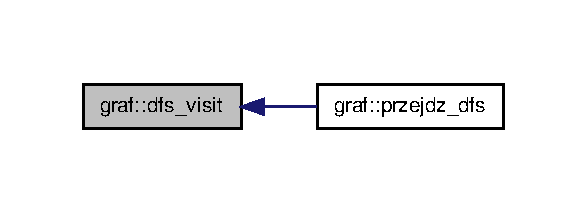
\includegraphics[width=282pt]{classgraf_a84527840c48cc131f9ef2ca493550ea0_icgraph}
\end{center}
\end{figure}


\hypertarget{classgraf_aa70de90b152f2cf47dac635793bcc5c4}{\index{graf@{graf}!dodaj\-\_\-polaczenie@{dodaj\-\_\-polaczenie}}
\index{dodaj\-\_\-polaczenie@{dodaj\-\_\-polaczenie}!graf@{graf}}
\subsubsection[{dodaj\-\_\-polaczenie}]{\setlength{\rightskip}{0pt plus 5cm}void {\bf graf\-::dodaj\-\_\-polaczenie} (
\begin{DoxyParamCaption}
\item[{int}]{v1, }
\item[{int}]{v2}
\end{DoxyParamCaption}
)}}\label{classgraf_aa70de90b152f2cf47dac635793bcc5c4}
funckcja sprawdza czy zadane wierzcholki zostaly utworzone jesli tak laczy je. 
\begin{DoxyParams}{\-Parameters}
{\em v1} & wierzcholki ktore maja zostac polaczone \\
\hline
{\em v2} & \\
\hline
\end{DoxyParams}


\-Definition at line 132 of file graf.\-cpp.



\-Here is the call graph for this function\-:\nopagebreak
\begin{figure}[H]
\begin{center}
\leavevmode
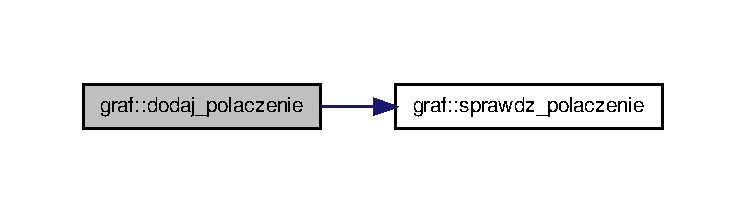
\includegraphics[width=350pt]{classgraf_aa70de90b152f2cf47dac635793bcc5c4_cgraph}
\end{center}
\end{figure}




\-Here is the caller graph for this function\-:\nopagebreak
\begin{figure}[H]
\begin{center}
\leavevmode
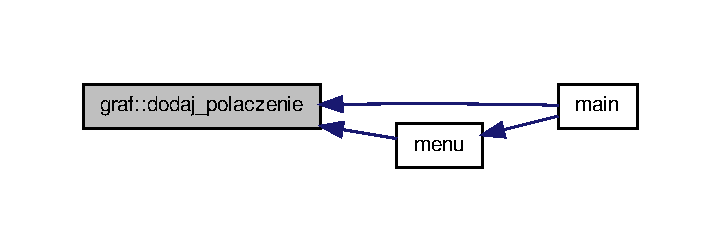
\includegraphics[width=346pt]{classgraf_aa70de90b152f2cf47dac635793bcc5c4_icgraph}
\end{center}
\end{figure}


\hypertarget{classgraf_a6a50b0bfb5fc3cfc7a443014170b9565}{\index{graf@{graf}!dodaj\-\_\-wierzcholek@{dodaj\-\_\-wierzcholek}}
\index{dodaj\-\_\-wierzcholek@{dodaj\-\_\-wierzcholek}!graf@{graf}}
\subsubsection[{dodaj\-\_\-wierzcholek}]{\setlength{\rightskip}{0pt plus 5cm}void {\bf graf\-::dodaj\-\_\-wierzcholek} (
\begin{DoxyParamCaption}
\item[{{\bf wierzcholek}}]{nowy}
\end{DoxyParamCaption}
)}}\label{classgraf_a6a50b0bfb5fc3cfc7a443014170b9565}

\begin{DoxyParams}{\-Parameters}
{\em nowy} & wierzcholek ktory ma zostac dodany \\
\hline
\end{DoxyParams}


\-Definition at line 52 of file graf.\-cpp.



\-Here is the caller graph for this function\-:\nopagebreak
\begin{figure}[H]
\begin{center}
\leavevmode
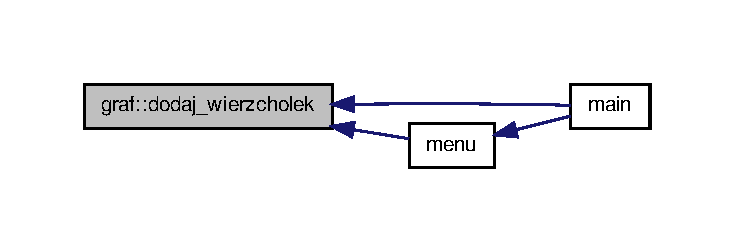
\includegraphics[width=350pt]{classgraf_a6a50b0bfb5fc3cfc7a443014170b9565_icgraph}
\end{center}
\end{figure}


\hypertarget{classgraf_afaa55f5a9aef1f30a2b3be97b59a476b}{\index{graf@{graf}!dodaj\-\_\-wierzcholek@{dodaj\-\_\-wierzcholek}}
\index{dodaj\-\_\-wierzcholek@{dodaj\-\_\-wierzcholek}!graf@{graf}}
\subsubsection[{dodaj\-\_\-wierzcholek}]{\setlength{\rightskip}{0pt plus 5cm}void {\bf graf\-::dodaj\-\_\-wierzcholek} (
\begin{DoxyParamCaption}
{}
\end{DoxyParamCaption}
)}}\label{classgraf_afaa55f5a9aef1f30a2b3be97b59a476b}
funkcja wymaga wprowadzania danych przez uzytkownika 

\-Definition at line 68 of file graf.\-cpp.

\hypertarget{classgraf_a5b67e5e829440e984782b232188a5f57}{\index{graf@{graf}!przejdz\-\_\-bfs@{przejdz\-\_\-bfs}}
\index{przejdz\-\_\-bfs@{przejdz\-\_\-bfs}!graf@{graf}}
\subsubsection[{przejdz\-\_\-bfs}]{\setlength{\rightskip}{0pt plus 5cm}{\bf element\-\_\-bfs} $\ast$ {\bf graf\-::przejdz\-\_\-bfs} (
\begin{DoxyParamCaption}
\item[{int}]{v1}
\end{DoxyParamCaption}
)}}\label{classgraf_a5b67e5e829440e984782b232188a5f57}
funkcja uzywa kolejki dostarczonej w \-S\-T\-L. wynikiem dzialania jest drzewo przejscia grafu zawierajace informacje o najkrutszych odleglosciach od korzenia 
\begin{DoxyParams}{\-Parameters}
{\em v1} & korzen przechodzenia \\
\hline
\end{DoxyParams}
\begin{DoxyReturn}{\-Returns}

\end{DoxyReturn}
kolorujemy korzen

petla wykonuje sie dopuki jest cis w kolejca 

\-Definition at line 189 of file graf.\-cpp.

\hypertarget{classgraf_a4947702a6d93feb805b1e11e14ec1e13}{\index{graf@{graf}!przejdz\-\_\-dfs@{przejdz\-\_\-dfs}}
\index{przejdz\-\_\-dfs@{przejdz\-\_\-dfs}!graf@{graf}}
\subsubsection[{przejdz\-\_\-dfs}]{\setlength{\rightskip}{0pt plus 5cm}void $\ast$ {\bf graf\-::przejdz\-\_\-dfs} (
\begin{DoxyParamCaption}
{}
\end{DoxyParamCaption}
)}}\label{classgraf_a4947702a6d93feb805b1e11e14ec1e13}
na ten moment wszystkie drzewa przechowywyane sa w jednej tablicy 

\-Definition at line 268 of file graf.\-cpp.



\-Here is the call graph for this function\-:
\nopagebreak
\begin{figure}[H]
\begin{center}
\leavevmode
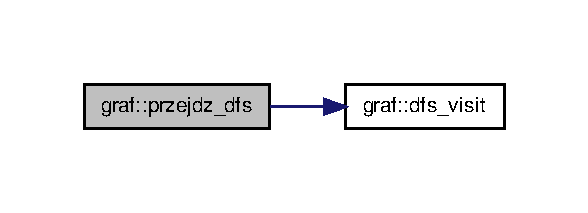
\includegraphics[width=282pt]{classgraf_a4947702a6d93feb805b1e11e14ec1e13_cgraph}
\end{center}
\end{figure}


\hypertarget{classgraf_ae1ebd85c7cb288174a5dccc5fd90634e}{\index{graf@{graf}!sprawdz\-\_\-polaczenie@{sprawdz\-\_\-polaczenie}}
\index{sprawdz\-\_\-polaczenie@{sprawdz\-\_\-polaczenie}!graf@{graf}}
\subsubsection[{sprawdz\-\_\-polaczenie}]{\setlength{\rightskip}{0pt plus 5cm}bool {\bf graf\-::sprawdz\-\_\-polaczenie} (
\begin{DoxyParamCaption}
\item[{int}]{v1, }
\item[{int}]{v2}
\end{DoxyParamCaption}
)}}\label{classgraf_ae1ebd85c7cb288174a5dccc5fd90634e}
funckcja sprawdza czy zadane wierzcholki zostaly utworzone nastepnie sprawdza polaczenie. 
\begin{DoxyParams}{\-Parameters}
{\em v1} & \\
\hline
{\em v2} & \\
\hline
\end{DoxyParams}
\begin{DoxyReturn}{\-Returns}
zwraca informacja logiczna 
\end{DoxyReturn}


\-Definition at line 158 of file graf.\-cpp.



\-Here is the caller graph for this function\-:\nopagebreak
\begin{figure}[H]
\begin{center}
\leavevmode
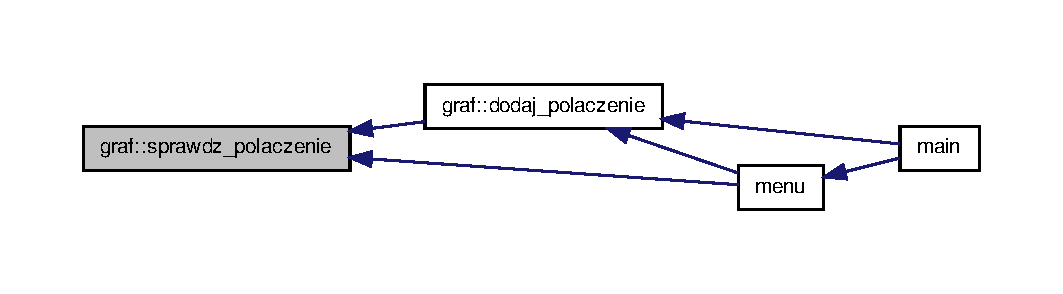
\includegraphics[width=350pt]{classgraf_ae1ebd85c7cb288174a5dccc5fd90634e_icgraph}
\end{center}
\end{figure}


\hypertarget{classgraf_ac7e01e940f136f4020e4da816c2fb1b4}{\index{graf@{graf}!usun\-\_\-polaczenie@{usun\-\_\-polaczenie}}
\index{usun\-\_\-polaczenie@{usun\-\_\-polaczenie}!graf@{graf}}
\subsubsection[{usun\-\_\-polaczenie}]{\setlength{\rightskip}{0pt plus 5cm}void {\bf graf\-::usun\-\_\-polaczenie} (
\begin{DoxyParamCaption}
\item[{int}]{v1, }
\item[{int}]{v2}
\end{DoxyParamCaption}
)}}\label{classgraf_ac7e01e940f136f4020e4da816c2fb1b4}

\begin{DoxyParams}{\-Parameters}
{\em v1} & wierzcholki ktorych polaczenie ma byc usuniete \\
\hline
{\em v2} & \\
\hline
\end{DoxyParams}


\-Definition at line 113 of file graf.\-cpp.



\-Here is the caller graph for this function\-:\nopagebreak
\begin{figure}[H]
\begin{center}
\leavevmode
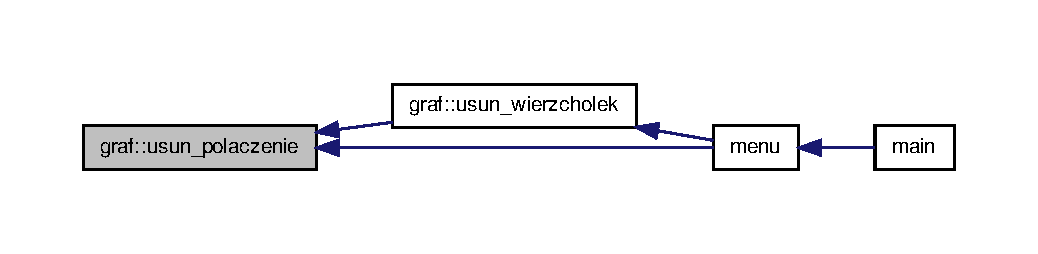
\includegraphics[width=350pt]{classgraf_ac7e01e940f136f4020e4da816c2fb1b4_icgraph}
\end{center}
\end{figure}


\hypertarget{classgraf_a369202eb63332e9faad779591c862ece}{\index{graf@{graf}!usun\-\_\-wierzcholek@{usun\-\_\-wierzcholek}}
\index{usun\-\_\-wierzcholek@{usun\-\_\-wierzcholek}!graf@{graf}}
\subsubsection[{usun\-\_\-wierzcholek}]{\setlength{\rightskip}{0pt plus 5cm}void {\bf graf\-::usun\-\_\-wierzcholek} (
\begin{DoxyParamCaption}
\item[{int}]{numer}
\end{DoxyParamCaption}
)}}\label{classgraf_a369202eb63332e9faad779591c862ece}

\begin{DoxyParams}{\-Parameters}
{\em numer} & klucz wierzcholka do usuniecia \\
\hline
\end{DoxyParams}


\-Definition at line 89 of file graf.\-cpp.



\-Here is the call graph for this function\-:\nopagebreak
\begin{figure}[H]
\begin{center}
\leavevmode
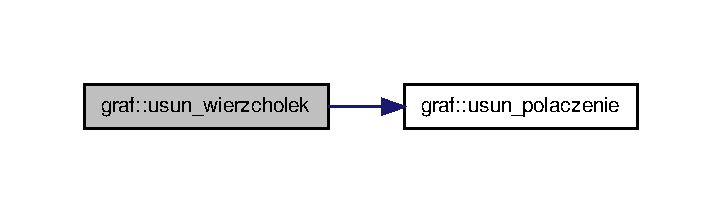
\includegraphics[width=346pt]{classgraf_a369202eb63332e9faad779591c862ece_cgraph}
\end{center}
\end{figure}




\-Here is the caller graph for this function\-:\nopagebreak
\begin{figure}[H]
\begin{center}
\leavevmode
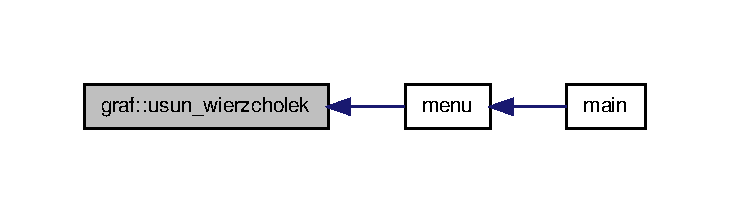
\includegraphics[width=350pt]{classgraf_a369202eb63332e9faad779591c862ece_icgraph}
\end{center}
\end{figure}


\hypertarget{classgraf_aa045d28e07e38ca32adf1b353077f877}{\index{graf@{graf}!wrozmiar@{wrozmiar}}
\index{wrozmiar@{wrozmiar}!graf@{graf}}
\subsubsection[{wrozmiar}]{\setlength{\rightskip}{0pt plus 5cm}int {\bf graf\-::wrozmiar} (
\begin{DoxyParamCaption}
{}
\end{DoxyParamCaption}
)}}\label{classgraf_aa045d28e07e38ca32adf1b353077f877}
\begin{DoxyReturn}{\-Returns}

\end{DoxyReturn}


\-Definition at line 103 of file graf.\-cpp.

\hypertarget{classgraf_a97c2722a11d3a7f90c82bc9b1cd56ef6}{\index{graf@{graf}!wyswietl\-\_\-dfs@{wyswietl\-\_\-dfs}}
\index{wyswietl\-\_\-dfs@{wyswietl\-\_\-dfs}!graf@{graf}}
\subsubsection[{wyswietl\-\_\-dfs}]{\setlength{\rightskip}{0pt plus 5cm}void {\bf graf\-::wyswietl\-\_\-dfs} (
\begin{DoxyParamCaption}
{}
\end{DoxyParamCaption}
)}}\label{classgraf_a97c2722a11d3a7f90c82bc9b1cd56ef6}


\-Definition at line 311 of file graf.\-cpp.

\hypertarget{classgraf_a8dd83fa1722d917a143b2da9245b5db9}{\index{graf@{graf}!wyswietl\-\_\-sasiadow@{wyswietl\-\_\-sasiadow}}
\index{wyswietl\-\_\-sasiadow@{wyswietl\-\_\-sasiadow}!graf@{graf}}
\subsubsection[{wyswietl\-\_\-sasiadow}]{\setlength{\rightskip}{0pt plus 5cm}void {\bf graf\-::wyswietl\-\_\-sasiadow} (
\begin{DoxyParamCaption}
\item[{int}]{numer}
\end{DoxyParamCaption}
)}}\label{classgraf_a8dd83fa1722d917a143b2da9245b5db9}
zostaje wyswietlona lista sasiedztwa 
\begin{DoxyParams}{\-Parameters}
{\em numer} & \\
\hline
\end{DoxyParams}


\-Definition at line 146 of file graf.\-cpp.



\-Here is the caller graph for this function\-:\nopagebreak
\begin{figure}[H]
\begin{center}
\leavevmode
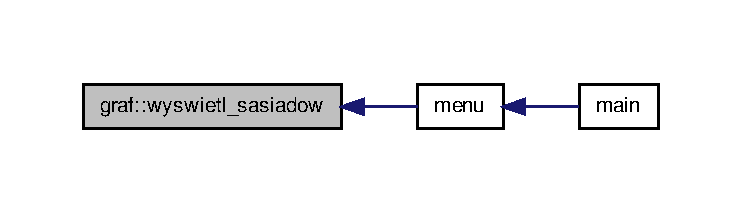
\includegraphics[width=350pt]{classgraf_a8dd83fa1722d917a143b2da9245b5db9_icgraph}
\end{center}
\end{figure}




\subsection{\-Friends \-And \-Related \-Function \-Documentation}
\hypertarget{classgraf_af2b2242aa53a3230ae67c7b57d7d9d11}{\index{graf@{graf}!bfs@{bfs}}
\index{bfs@{bfs}!graf@{graf}}
\subsubsection[{bfs}]{\setlength{\rightskip}{0pt plus 5cm}friend class {\bf bfs}\hspace{0.3cm}{\ttfamily  \mbox{[}friend\mbox{]}}}}\label{classgraf_af2b2242aa53a3230ae67c7b57d7d9d11}


\-Definition at line 49 of file graf.\-hh.

\hypertarget{classgraf_aaf525f8cdadbe40d9ad7c39f79fd8a2c}{\index{graf@{graf}!operator$<$$<$@{operator$<$$<$}}
\index{operator$<$$<$@{operator$<$$<$}!graf@{graf}}
\subsubsection[{operator$<$$<$}]{\setlength{\rightskip}{0pt plus 5cm}ostream\& operator$<$$<$ (
\begin{DoxyParamCaption}
\item[{ostream \&}]{wyjscie, }
\item[{{\bf graf} \&}]{dane}
\end{DoxyParamCaption}
)\hspace{0.3cm}{\ttfamily  \mbox{[}friend\mbox{]}}}}\label{classgraf_aaf525f8cdadbe40d9ad7c39f79fd8a2c}

\begin{DoxyParams}{\-Parameters}
{\em wyjscie} & strumien wyjscia \\
\hline
{\em dane} & wysylane dane \\
\hline
\end{DoxyParams}


\-Definition at line 15 of file graf.\-cpp.



\subsection{\-Member \-Data \-Documentation}
\hypertarget{classgraf_ad9204c0bbc75a2bef4a43200672f9694}{\index{graf@{graf}!ilosc@{ilosc}}
\index{ilosc@{ilosc}!graf@{graf}}
\subsubsection[{ilosc}]{\setlength{\rightskip}{0pt plus 5cm}int {\bf graf\-::ilosc}\hspace{0.3cm}{\ttfamily  \mbox{[}private\mbox{]}}}}\label{classgraf_ad9204c0bbc75a2bef4a43200672f9694}


\-Definition at line 31 of file graf.\-hh.

\hypertarget{classgraf_a596da8a77b680d7ec408b1253c2c43c3}{\index{graf@{graf}!rozmiar@{rozmiar}}
\index{rozmiar@{rozmiar}!graf@{graf}}
\subsubsection[{rozmiar}]{\setlength{\rightskip}{0pt plus 5cm}int {\bf graf\-::rozmiar}\hspace{0.3cm}{\ttfamily  \mbox{[}private\mbox{]}}}}\label{classgraf_a596da8a77b680d7ec408b1253c2c43c3}


\-Definition at line 30 of file graf.\-hh.

\hypertarget{classgraf_a028d547c797438718da6241a28b32db5}{\index{graf@{graf}!tablica@{tablica}}
\index{tablica@{tablica}!graf@{graf}}
\subsubsection[{tablica}]{\setlength{\rightskip}{0pt plus 5cm}{\bf wierzcholek}$\ast$ {\bf graf\-::tablica}\hspace{0.3cm}{\ttfamily  \mbox{[}private\mbox{]}}}}\label{classgraf_a028d547c797438718da6241a28b32db5}


\-Definition at line 29 of file graf.\-hh.

\hypertarget{classgraf_a325616745236599f83bffb58d61b0fa9}{\index{graf@{graf}!tablica\-\_\-dfs@{tablica\-\_\-dfs}}
\index{tablica\-\_\-dfs@{tablica\-\_\-dfs}!graf@{graf}}
\subsubsection[{tablica\-\_\-dfs}]{\setlength{\rightskip}{0pt plus 5cm}{\bf element\-\_\-dfs}$\ast$ {\bf graf\-::tablica\-\_\-dfs}\hspace{0.3cm}{\ttfamily  \mbox{[}private\mbox{]}}}}\label{classgraf_a325616745236599f83bffb58d61b0fa9}


\-Definition at line 33 of file graf.\-hh.

\hypertarget{classgraf_a9202cb6ab351f5bbdbb79de440ab1fb5}{\index{graf@{graf}!time@{time}}
\index{time@{time}!graf@{graf}}
\subsubsection[{time}]{\setlength{\rightskip}{0pt plus 5cm}int {\bf graf\-::time}\hspace{0.3cm}{\ttfamily  \mbox{[}private\mbox{]}}}}\label{classgraf_a9202cb6ab351f5bbdbb79de440ab1fb5}


\-Definition at line 32 of file graf.\-hh.



\-The documentation for this class was generated from the following files\-:\begin{DoxyCompactItemize}
\item 
prj/\hyperlink{graf_8hh}{graf.\-hh}\item 
prj/\hyperlink{graf_8cpp}{graf.\-cpp}\end{DoxyCompactItemize}

\hypertarget{structpolaczenie}{\section{polaczenie \-Struct \-Reference}
\label{structpolaczenie}\index{polaczenie@{polaczenie}}
}


struktura modeluje pojecie polaczenia wierzcholkow grafu  




{\ttfamily \#include $<$wierzcholek.\-hh$>$}

\subsection*{\-Public \-Member \-Functions}
\begin{DoxyCompactItemize}
\item 
\hyperlink{structpolaczenie_ab05efb1d31231883dca69f9067a5cfaf}{polaczenie} ()
\item 
\hyperlink{structpolaczenie}{polaczenie} \hyperlink{structpolaczenie_aa16901afdb430c2cb37142fbd90b7c03}{operator+} (\hyperlink{structpolaczenie}{polaczenie} element)
\end{DoxyCompactItemize}
\subsection*{\-Public \-Attributes}
\begin{DoxyCompactItemize}
\item 
int \hyperlink{structpolaczenie_a9faa3298bef8b4c35a1897caad57f2b0}{wierzcholek}
\item 
int \hyperlink{structpolaczenie_a3cf76ce70d5eea1c5d96abd57f737ff2}{waga}
\end{DoxyCompactItemize}


\subsection{\-Detailed \-Description}


\-Definition at line 22 of file wierzcholek.\-hh.



\subsection{\-Constructor \& \-Destructor \-Documentation}
\hypertarget{structpolaczenie_ab05efb1d31231883dca69f9067a5cfaf}{\index{polaczenie@{polaczenie}!polaczenie@{polaczenie}}
\index{polaczenie@{polaczenie}!polaczenie@{polaczenie}}
\subsubsection[{polaczenie}]{\setlength{\rightskip}{0pt plus 5cm}{\bf polaczenie\-::polaczenie} (
\begin{DoxyParamCaption}
{}
\end{DoxyParamCaption}
)\hspace{0.3cm}{\ttfamily  \mbox{[}inline\mbox{]}}}}\label{structpolaczenie_ab05efb1d31231883dca69f9067a5cfaf}


\-Definition at line 26 of file wierzcholek.\-hh.



\subsection{\-Member \-Function \-Documentation}
\hypertarget{structpolaczenie_aa16901afdb430c2cb37142fbd90b7c03}{\index{polaczenie@{polaczenie}!operator+@{operator+}}
\index{operator+@{operator+}!polaczenie@{polaczenie}}
\subsubsection[{operator+}]{\setlength{\rightskip}{0pt plus 5cm}{\bf polaczenie} polaczenie\-::operator+ (
\begin{DoxyParamCaption}
\item[{{\bf polaczenie}}]{element}
\end{DoxyParamCaption}
)\hspace{0.3cm}{\ttfamily  \mbox{[}inline\mbox{]}}}}\label{structpolaczenie_aa16901afdb430c2cb37142fbd90b7c03}


\-Definition at line 30 of file wierzcholek.\-hh.



\subsection{\-Member \-Data \-Documentation}
\hypertarget{structpolaczenie_a3cf76ce70d5eea1c5d96abd57f737ff2}{\index{polaczenie@{polaczenie}!waga@{waga}}
\index{waga@{waga}!polaczenie@{polaczenie}}
\subsubsection[{waga}]{\setlength{\rightskip}{0pt plus 5cm}int {\bf polaczenie\-::waga}}}\label{structpolaczenie_a3cf76ce70d5eea1c5d96abd57f737ff2}


\-Definition at line 25 of file wierzcholek.\-hh.

\hypertarget{structpolaczenie_a9faa3298bef8b4c35a1897caad57f2b0}{\index{polaczenie@{polaczenie}!wierzcholek@{wierzcholek}}
\index{wierzcholek@{wierzcholek}!polaczenie@{polaczenie}}
\subsubsection[{wierzcholek}]{\setlength{\rightskip}{0pt plus 5cm}int {\bf polaczenie\-::wierzcholek}}}\label{structpolaczenie_a9faa3298bef8b4c35a1897caad57f2b0}


\-Definition at line 24 of file wierzcholek.\-hh.



\-The documentation for this struct was generated from the following file\-:\begin{DoxyCompactItemize}
\item 
prj/\hyperlink{wierzcholek_8hh}{wierzcholek.\-hh}\end{DoxyCompactItemize}

\hypertarget{classwierzcholek}{\section{wierzcholek \-Class \-Reference}
\label{classwierzcholek}\index{wierzcholek@{wierzcholek}}
}


{\ttfamily \#include $<$wierzcholek.\-hh$>$}

\subsection*{\-Public \-Member \-Functions}
\begin{DoxyCompactItemize}
\item 
\hyperlink{classwierzcholek_a0e72695b032e7f750c51041e1a59673b}{wierzcholek} ()
\begin{DoxyCompactList}\small\item\em konstruktor \end{DoxyCompactList}\end{DoxyCompactItemize}
\subsection*{\-Public \-Attributes}
\begin{DoxyCompactItemize}
\item 
bool \hyperlink{classwierzcholek_ad67644b5f408397f28d7150d3bac76d2}{zajety}
\end{DoxyCompactItemize}
\subsection*{\-Private \-Attributes}
\begin{DoxyCompactItemize}
\item 
int \hyperlink{classwierzcholek_a66aaea6b1187250f7100542adc1617d2}{numer}
\item 
string \hyperlink{classwierzcholek_a19aa16bf7e01a987fcc360e5da902209}{wartosc}
\begin{DoxyCompactList}\small\item\em identyfikator wierzcholka \end{DoxyCompactList}\item 
vector$<$ \hyperlink{structpolaczenie}{polaczenie} $>$ \hyperlink{classwierzcholek_ad6442177753c61769b0fa1822e75f551}{polaczenia}
\begin{DoxyCompactList}\small\item\em wartosc przechowywana w wierzcholku \end{DoxyCompactList}\end{DoxyCompactItemize}
\subsection*{\-Friends}
\begin{DoxyCompactItemize}
\item 
class \hyperlink{classwierzcholek_a1726ca1919686bdccbca505bacf6de2f}{graf}
\begin{DoxyCompactList}\small\item\em zmienna okresla czy wierzcholek zostal zdefiniowany \end{DoxyCompactList}\item 
ostream \& \hyperlink{classwierzcholek_ab0941004cc1a9bb9339cf2092b1819a1}{operator$<$$<$} (ostream \&wyjscie, \hyperlink{classwierzcholek}{wierzcholek} \&wej)
\begin{DoxyCompactList}\small\item\em lista polaczen wierzcholka \end{DoxyCompactList}\item 
istream \& \hyperlink{classwierzcholek_a221c2b565a9506a8eaed69e42e374f4e}{operator$>$$>$} (istream \&wejscie, \hyperlink{classwierzcholek}{wierzcholek} \&wyj)
\end{DoxyCompactItemize}


\subsection{\-Detailed \-Description}


\-Definition at line 39 of file wierzcholek.\-hh.



\subsection{\-Constructor \& \-Destructor \-Documentation}
\hypertarget{classwierzcholek_a0e72695b032e7f750c51041e1a59673b}{\index{wierzcholek@{wierzcholek}!wierzcholek@{wierzcholek}}
\index{wierzcholek@{wierzcholek}!wierzcholek@{wierzcholek}}
\subsubsection[{wierzcholek}]{\setlength{\rightskip}{0pt plus 5cm}{\bf wierzcholek\-::wierzcholek} (
\begin{DoxyParamCaption}
{}
\end{DoxyParamCaption}
)\hspace{0.3cm}{\ttfamily  \mbox{[}inline\mbox{]}}}}\label{classwierzcholek_a0e72695b032e7f750c51041e1a59673b}


\-Definition at line 51 of file wierzcholek.\-hh.



\subsection{\-Friends \-And \-Related \-Function \-Documentation}
\hypertarget{classwierzcholek_a1726ca1919686bdccbca505bacf6de2f}{\index{wierzcholek@{wierzcholek}!graf@{graf}}
\index{graf@{graf}!wierzcholek@{wierzcholek}}
\subsubsection[{graf}]{\setlength{\rightskip}{0pt plus 5cm}friend class {\bf graf}\hspace{0.3cm}{\ttfamily  \mbox{[}friend\mbox{]}}}}\label{classwierzcholek_a1726ca1919686bdccbca505bacf6de2f}


\-Definition at line 49 of file wierzcholek.\-hh.

\hypertarget{classwierzcholek_ab0941004cc1a9bb9339cf2092b1819a1}{\index{wierzcholek@{wierzcholek}!operator$<$$<$@{operator$<$$<$}}
\index{operator$<$$<$@{operator$<$$<$}!wierzcholek@{wierzcholek}}
\subsubsection[{operator$<$$<$}]{\setlength{\rightskip}{0pt plus 5cm}ostream\& operator$<$$<$ (
\begin{DoxyParamCaption}
\item[{ostream \&}]{wyjscie, }
\item[{{\bf wierzcholek} \&}]{wej}
\end{DoxyParamCaption}
)\hspace{0.3cm}{\ttfamily  \mbox{[}friend\mbox{]}}}}\label{classwierzcholek_ab0941004cc1a9bb9339cf2092b1819a1}


\-Definition at line 17 of file wierzcholek.\-cpp.

\hypertarget{classwierzcholek_a221c2b565a9506a8eaed69e42e374f4e}{\index{wierzcholek@{wierzcholek}!operator$>$$>$@{operator$>$$>$}}
\index{operator$>$$>$@{operator$>$$>$}!wierzcholek@{wierzcholek}}
\subsubsection[{operator$>$$>$}]{\setlength{\rightskip}{0pt plus 5cm}istream\& operator$>$$>$ (
\begin{DoxyParamCaption}
\item[{istream \&}]{wejscie, }
\item[{{\bf wierzcholek} \&}]{wyj}
\end{DoxyParamCaption}
)\hspace{0.3cm}{\ttfamily  \mbox{[}friend\mbox{]}}}}\label{classwierzcholek_a221c2b565a9506a8eaed69e42e374f4e}


\-Definition at line 32 of file wierzcholek.\-cpp.



\subsection{\-Member \-Data \-Documentation}
\hypertarget{classwierzcholek_a66aaea6b1187250f7100542adc1617d2}{\index{wierzcholek@{wierzcholek}!numer@{numer}}
\index{numer@{numer}!wierzcholek@{wierzcholek}}
\subsubsection[{numer}]{\setlength{\rightskip}{0pt plus 5cm}int {\bf wierzcholek\-::numer}\hspace{0.3cm}{\ttfamily  \mbox{[}private\mbox{]}}}}\label{classwierzcholek_a66aaea6b1187250f7100542adc1617d2}


\-Definition at line 42 of file wierzcholek.\-hh.

\hypertarget{classwierzcholek_ad6442177753c61769b0fa1822e75f551}{\index{wierzcholek@{wierzcholek}!polaczenia@{polaczenia}}
\index{polaczenia@{polaczenia}!wierzcholek@{wierzcholek}}
\subsubsection[{polaczenia}]{\setlength{\rightskip}{0pt plus 5cm}vector$<${\bf polaczenie}$>$ {\bf wierzcholek\-::polaczenia}\hspace{0.3cm}{\ttfamily  \mbox{[}private\mbox{]}}}}\label{classwierzcholek_ad6442177753c61769b0fa1822e75f551}


\-Definition at line 44 of file wierzcholek.\-hh.

\hypertarget{classwierzcholek_a19aa16bf7e01a987fcc360e5da902209}{\index{wierzcholek@{wierzcholek}!wartosc@{wartosc}}
\index{wartosc@{wartosc}!wierzcholek@{wierzcholek}}
\subsubsection[{wartosc}]{\setlength{\rightskip}{0pt plus 5cm}string {\bf wierzcholek\-::wartosc}\hspace{0.3cm}{\ttfamily  \mbox{[}private\mbox{]}}}}\label{classwierzcholek_a19aa16bf7e01a987fcc360e5da902209}


\-Definition at line 43 of file wierzcholek.\-hh.

\hypertarget{classwierzcholek_ad67644b5f408397f28d7150d3bac76d2}{\index{wierzcholek@{wierzcholek}!zajety@{zajety}}
\index{zajety@{zajety}!wierzcholek@{wierzcholek}}
\subsubsection[{zajety}]{\setlength{\rightskip}{0pt plus 5cm}bool {\bf wierzcholek\-::zajety}}}\label{classwierzcholek_ad67644b5f408397f28d7150d3bac76d2}


\-Definition at line 48 of file wierzcholek.\-hh.



\-The documentation for this class was generated from the following file\-:\begin{DoxyCompactItemize}
\item 
prj/\hyperlink{wierzcholek_8hh}{wierzcholek.\-hh}\end{DoxyCompactItemize}

\chapter{\-File \-Documentation}
\hypertarget{generator_8cpp}{\section{prj/generator.cpp \-File \-Reference}
\label{generator_8cpp}\index{prj/generator.\-cpp@{prj/generator.\-cpp}}
}
{\ttfamily \#include \char`\"{}generator.\-hh\char`\"{}}\*
\-Include dependency graph for generator.\-cpp\-:\nopagebreak
\begin{figure}[H]
\begin{center}
\leavevmode
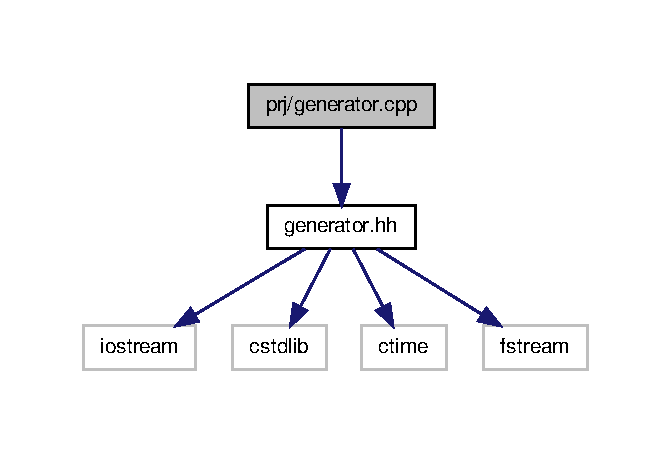
\includegraphics[width=322pt]{generator_8cpp__incl}
\end{center}
\end{figure}
\subsection*{\-Functions}
\begin{DoxyCompactItemize}
\item 
void \hyperlink{generator_8cpp_a242a9701c409c59f651874736f8cef01}{generuj\-\_\-polaczenia} (int rozmiar)
\begin{DoxyCompactList}\small\item\em generuje plik $\ast$.txt o zadanej ilosci danych i nazwie \end{DoxyCompactList}\item 
void \hyperlink{generator_8cpp_ae448f3fbbbd7702dc3faea2a133947d8}{generuj\-\_\-wierzcholki} (int rozmiar)
\end{DoxyCompactItemize}


\subsection{\-Function \-Documentation}
\hypertarget{generator_8cpp_a242a9701c409c59f651874736f8cef01}{\index{generator.\-cpp@{generator.\-cpp}!generuj\-\_\-polaczenia@{generuj\-\_\-polaczenia}}
\index{generuj\-\_\-polaczenia@{generuj\-\_\-polaczenia}!generator.cpp@{generator.\-cpp}}
\subsubsection[{generuj\-\_\-polaczenia}]{\setlength{\rightskip}{0pt plus 5cm}void {\bf generuj\-\_\-polaczenia} (
\begin{DoxyParamCaption}
\item[{int}]{rozmiar}
\end{DoxyParamCaption}
)}}\label{generator_8cpp_a242a9701c409c59f651874736f8cef01}
\-W pliku umieszczane sa liczby naturalne od 1 wzwyrz w pierwszym wierszu umieszczana jest liczba mowiaca o ilosci wierszy danych. 
\begin{DoxyParams}{\-Parameters}
{\em nazwa} & -\/ utworzonego pliku \\
\hline
{\em rozmiar} & -\/ ilosc wierszy sanych \\
\hline
\end{DoxyParams}


\-Definition at line 19 of file generator.\-cpp.

\hypertarget{generator_8cpp_ae448f3fbbbd7702dc3faea2a133947d8}{\index{generator.\-cpp@{generator.\-cpp}!generuj\-\_\-wierzcholki@{generuj\-\_\-wierzcholki}}
\index{generuj\-\_\-wierzcholki@{generuj\-\_\-wierzcholki}!generator.cpp@{generator.\-cpp}}
\subsubsection[{generuj\-\_\-wierzcholki}]{\setlength{\rightskip}{0pt plus 5cm}void {\bf generuj\-\_\-wierzcholki} (
\begin{DoxyParamCaption}
\item[{int}]{rozmiar}
\end{DoxyParamCaption}
)}}\label{generator_8cpp_ae448f3fbbbd7702dc3faea2a133947d8}


\-Definition at line 32 of file generator.\-cpp.


\hypertarget{generator_8hh}{\section{prj/generator.hh \-File \-Reference}
\label{generator_8hh}\index{prj/generator.\-hh@{prj/generator.\-hh}}
}
{\ttfamily \#include $<$iostream$>$}\*
{\ttfamily \#include $<$cstdlib$>$}\*
{\ttfamily \#include $<$ctime$>$}\*
{\ttfamily \#include $<$fstream$>$}\*
\-Include dependency graph for generator.\-hh\-:\nopagebreak
\begin{figure}[H]
\begin{center}
\leavevmode
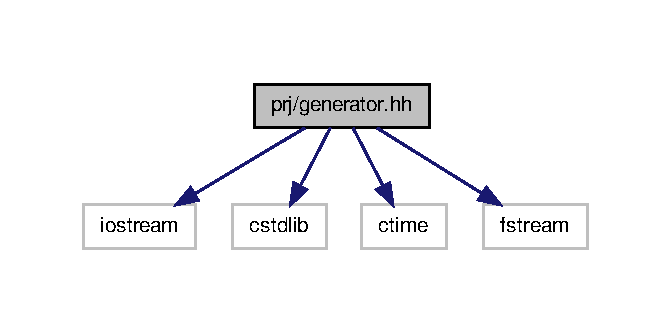
\includegraphics[width=322pt]{generator_8hh__incl}
\end{center}
\end{figure}
\-This graph shows which files directly or indirectly include this file\-:\nopagebreak
\begin{figure}[H]
\begin{center}
\leavevmode
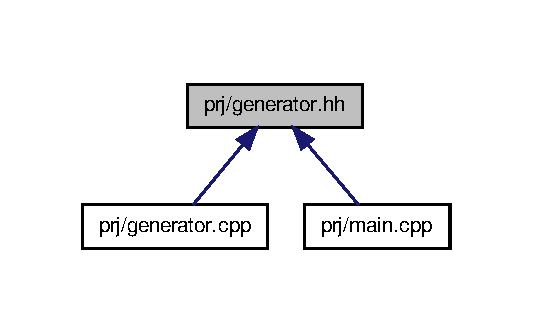
\includegraphics[width=256pt]{generator_8hh__dep__incl}
\end{center}
\end{figure}
\subsection*{\-Functions}
\begin{DoxyCompactItemize}
\item 
void \hyperlink{generator_8hh_a242a9701c409c59f651874736f8cef01}{generuj\-\_\-polaczenia} (int rozmiar)
\begin{DoxyCompactList}\small\item\em generuje plik $\ast$.txt o zadanej ilosci polaczen. \end{DoxyCompactList}\item 
void \hyperlink{generator_8hh_ae448f3fbbbd7702dc3faea2a133947d8}{generuj\-\_\-wierzcholki} (int rozmiar)
\end{DoxyCompactItemize}


\subsection{\-Function \-Documentation}
\hypertarget{generator_8hh_a242a9701c409c59f651874736f8cef01}{\index{generator.\-hh@{generator.\-hh}!generuj\-\_\-polaczenia@{generuj\-\_\-polaczenia}}
\index{generuj\-\_\-polaczenia@{generuj\-\_\-polaczenia}!generator.hh@{generator.\-hh}}
\subsubsection[{generuj\-\_\-polaczenia}]{\setlength{\rightskip}{0pt plus 5cm}void {\bf generuj\-\_\-polaczenia} (
\begin{DoxyParamCaption}
\item[{int}]{rozmiar}
\end{DoxyParamCaption}
)}}\label{generator_8hh_a242a9701c409c59f651874736f8cef01}
polaczenia sa generowane maxymalnie miedzy wierzcholkiem oddalonym o 6. 
\begin{DoxyParams}{\-Parameters}
{\em nazwa} & -\/ utworzonego pliku \\
\hline
{\em rozmiar} & -\/ ilosc wierszy sanych \\
\hline
\end{DoxyParams}


\-Definition at line 18 of file generator.\-cpp.



\-Here is the caller graph for this function\-:\nopagebreak
\begin{figure}[H]
\begin{center}
\leavevmode
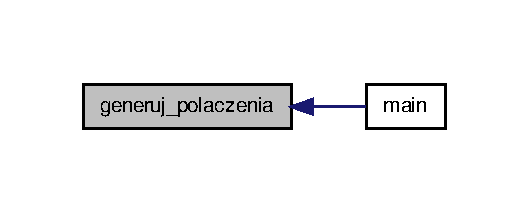
\includegraphics[width=254pt]{generator_8hh_a242a9701c409c59f651874736f8cef01_icgraph}
\end{center}
\end{figure}


\hypertarget{generator_8hh_ae448f3fbbbd7702dc3faea2a133947d8}{\index{generator.\-hh@{generator.\-hh}!generuj\-\_\-wierzcholki@{generuj\-\_\-wierzcholki}}
\index{generuj\-\_\-wierzcholki@{generuj\-\_\-wierzcholki}!generator.hh@{generator.\-hh}}
\subsubsection[{generuj\-\_\-wierzcholki}]{\setlength{\rightskip}{0pt plus 5cm}void {\bf generuj\-\_\-wierzcholki} (
\begin{DoxyParamCaption}
\item[{int}]{rozmiar}
\end{DoxyParamCaption}
)}}\label{generator_8hh_ae448f3fbbbd7702dc3faea2a133947d8}


\-Definition at line 42 of file generator.\-cpp.


\hypertarget{graf_8cpp}{\section{prj/graf.cpp \-File \-Reference}
\label{graf_8cpp}\index{prj/graf.\-cpp@{prj/graf.\-cpp}}
}
{\ttfamily \#include \char`\"{}graf.\-hh\char`\"{}}\*
\-Include dependency graph for graf.\-cpp\-:
\nopagebreak
\begin{figure}[H]
\begin{center}
\leavevmode
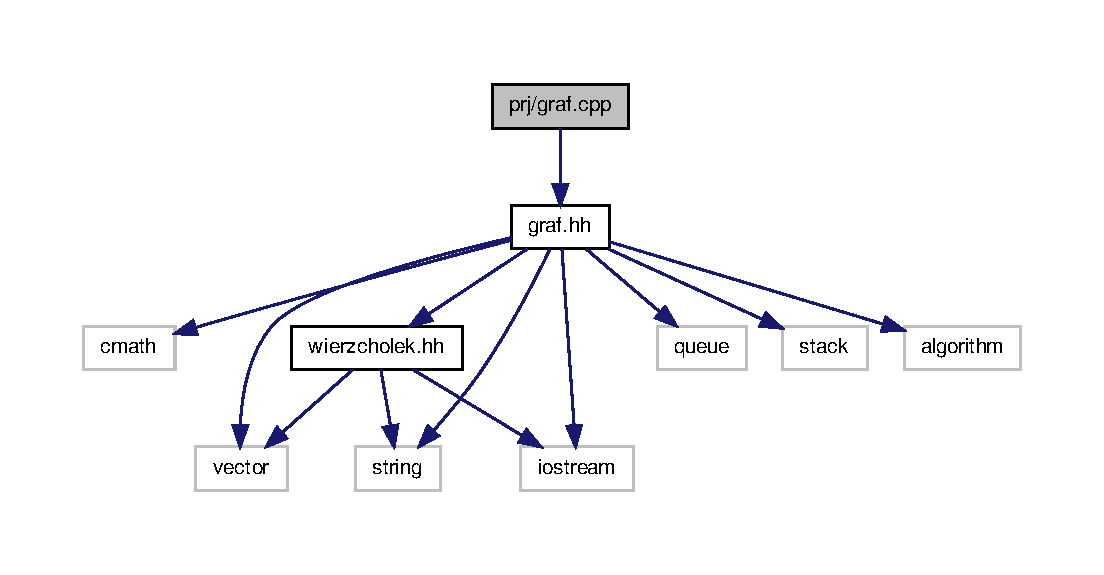
\includegraphics[width=350pt]{graf_8cpp__incl}
\end{center}
\end{figure}
\subsection*{\-Functions}
\begin{DoxyCompactItemize}
\item 
ostream \& \hyperlink{graf_8cpp_aaf525f8cdadbe40d9ad7c39f79fd8a2c}{operator$<$$<$} (ostream \&wyjscie, \hyperlink{classgraf}{graf} \&dane)
\begin{DoxyCompactList}\small\item\em przeladowanie operatora wyjscia \end{DoxyCompactList}\end{DoxyCompactItemize}


\subsection{\-Function \-Documentation}
\hypertarget{graf_8cpp_aaf525f8cdadbe40d9ad7c39f79fd8a2c}{\index{graf.\-cpp@{graf.\-cpp}!operator$<$$<$@{operator$<$$<$}}
\index{operator$<$$<$@{operator$<$$<$}!graf.cpp@{graf.\-cpp}}
\subsubsection[{operator$<$$<$}]{\setlength{\rightskip}{0pt plus 5cm}ostream\& operator$<$$<$ (
\begin{DoxyParamCaption}
\item[{ostream \&}]{wyjscie, }
\item[{{\bf graf} \&}]{dane}
\end{DoxyParamCaption}
)}}\label{graf_8cpp_aaf525f8cdadbe40d9ad7c39f79fd8a2c}

\begin{DoxyParams}{\-Parameters}
{\em wyjscie} & strumien wyjscia \\
\hline
{\em dane} & wysylane dane \\
\hline
\end{DoxyParams}


\-Definition at line 15 of file graf.\-cpp.


\hypertarget{graf_8hh}{\section{prj/graf.hh \-File \-Reference}
\label{graf_8hh}\index{prj/graf.\-hh@{prj/graf.\-hh}}
}
{\ttfamily \#include $<$cmath$>$}\*
{\ttfamily \#include $<$vector$>$}\*
{\ttfamily \#include $<$string$>$}\*
{\ttfamily \#include $<$iostream$>$}\*
{\ttfamily \#include \char`\"{}wierzcholek.\-hh\char`\"{}}\*
{\ttfamily \#include $<$queue$>$}\*
{\ttfamily \#include $<$stack$>$}\*
{\ttfamily \#include $<$algorithm$>$}\*
\-Include dependency graph for graf.\-hh\-:
\nopagebreak
\begin{figure}[H]
\begin{center}
\leavevmode
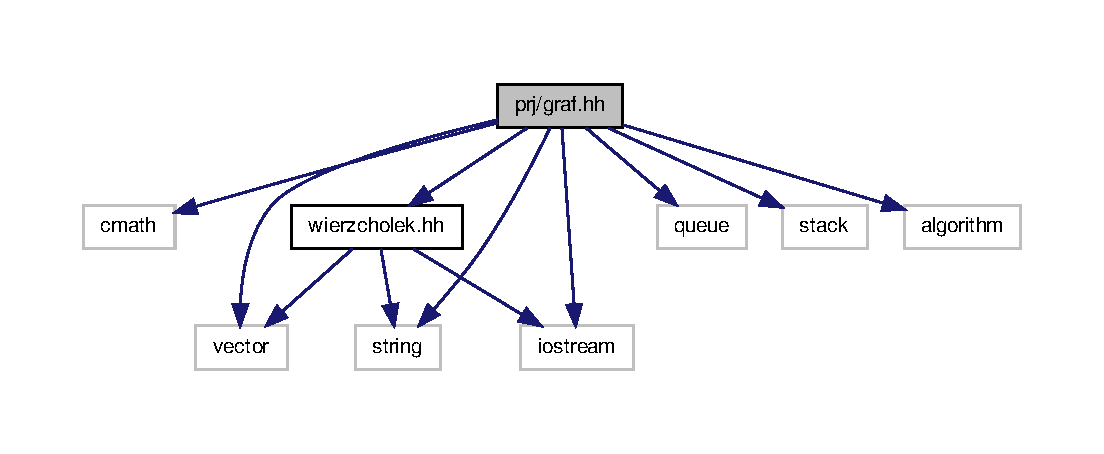
\includegraphics[width=350pt]{graf_8hh__incl}
\end{center}
\end{figure}
\-This graph shows which files directly or indirectly include this file\-:\nopagebreak
\begin{figure}[H]
\begin{center}
\leavevmode
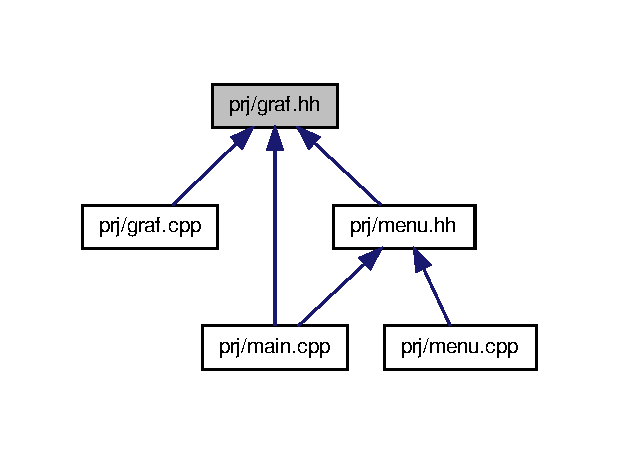
\includegraphics[width=297pt]{graf_8hh__dep__incl}
\end{center}
\end{figure}
\subsection*{\-Classes}
\begin{DoxyCompactItemize}
\item 
class \hyperlink{classgraf}{graf}
\begin{DoxyCompactList}\small\item\em klasa modeluje graf. \end{DoxyCompactList}\end{DoxyCompactItemize}

\hypertarget{komiwojazer_8cpp}{\section{prj/komiwojazer.cpp \-File \-Reference}
\label{komiwojazer_8cpp}\index{prj/komiwojazer.\-cpp@{prj/komiwojazer.\-cpp}}
}
{\ttfamily \#include \char`\"{}komiwojazer.\-hh\char`\"{}}\*
\-Include dependency graph for komiwojazer.\-cpp\-:
\nopagebreak
\begin{figure}[H]
\begin{center}
\leavevmode
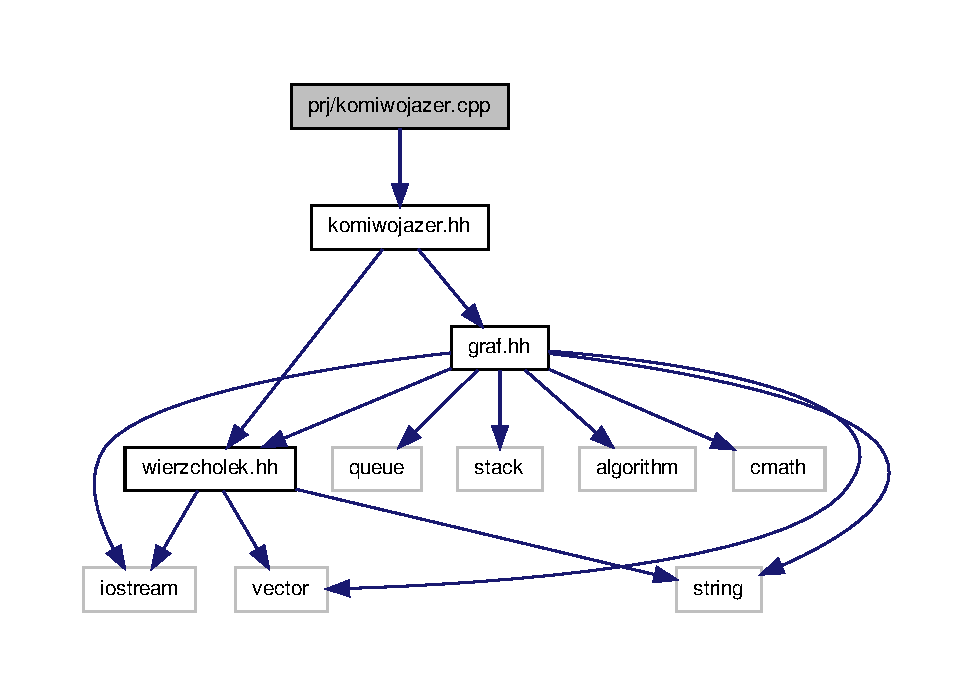
\includegraphics[width=350pt]{komiwojazer_8cpp__incl}
\end{center}
\end{figure}

\hypertarget{komiwojazer_8hh}{\section{prj/komiwojazer.hh \-File \-Reference}
\label{komiwojazer_8hh}\index{prj/komiwojazer.\-hh@{prj/komiwojazer.\-hh}}
}
{\ttfamily \#include \char`\"{}graf.\-hh\char`\"{}}\*
{\ttfamily \#include \char`\"{}wierzcholek.\-hh\char`\"{}}\*
\-Include dependency graph for komiwojazer.\-hh\-:
\nopagebreak
\begin{figure}[H]
\begin{center}
\leavevmode
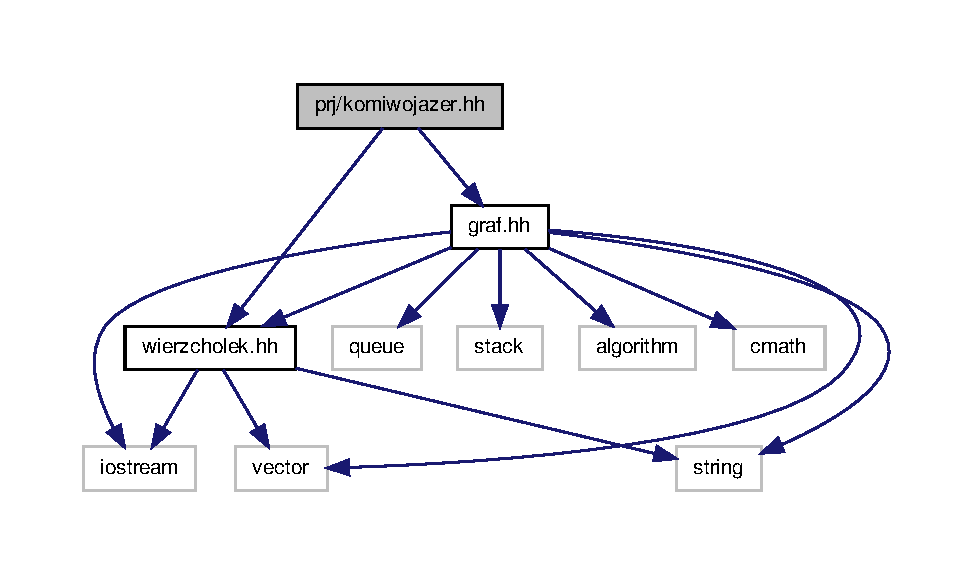
\includegraphics[width=350pt]{komiwojazer_8hh__incl}
\end{center}
\end{figure}
\-This graph shows which files directly or indirectly include this file\-:
\nopagebreak
\begin{figure}[H]
\begin{center}
\leavevmode
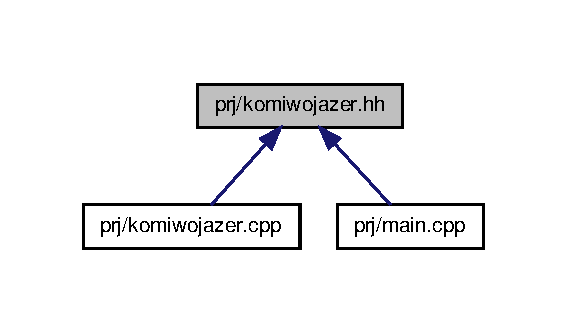
\includegraphics[width=272pt]{komiwojazer_8hh__dep__incl}
\end{center}
\end{figure}
\subsection*{\-Classes}
\begin{DoxyCompactItemize}
\item 
struct \hyperlink{structelement__komi}{element\-\_\-komi}
\begin{DoxyCompactList}\small\item\em klasa modeluje element drogi komiwojazera \end{DoxyCompactList}\item 
class \hyperlink{classdroga__komi}{droga\-\_\-komi}
\begin{DoxyCompactList}\small\item\em klasa modeluje pojecie drogi komiwojazera. \end{DoxyCompactList}\end{DoxyCompactItemize}

\hypertarget{main_8cpp}{\section{prj/main.cpp \-File \-Reference}
\label{main_8cpp}\index{prj/main.\-cpp@{prj/main.\-cpp}}
}
{\ttfamily \#include $<$iostream$>$}\*
{\ttfamily \#include $<$fstream$>$}\*
{\ttfamily \#include $<$string$>$}\*
{\ttfamily \#include \char`\"{}graf.\-hh\char`\"{}}\*
{\ttfamily \#include \char`\"{}wierzcholek.\-hh\char`\"{}}\*
{\ttfamily \#include \char`\"{}generator.\-hh\char`\"{}}\*
{\ttfamily \#include \char`\"{}menu.\-hh\char`\"{}}\*
{\ttfamily \#include \char`\"{}stoper.\-hh\char`\"{}}\*
\-Include dependency graph for main.\-cpp\-:
\nopagebreak
\begin{figure}[H]
\begin{center}
\leavevmode
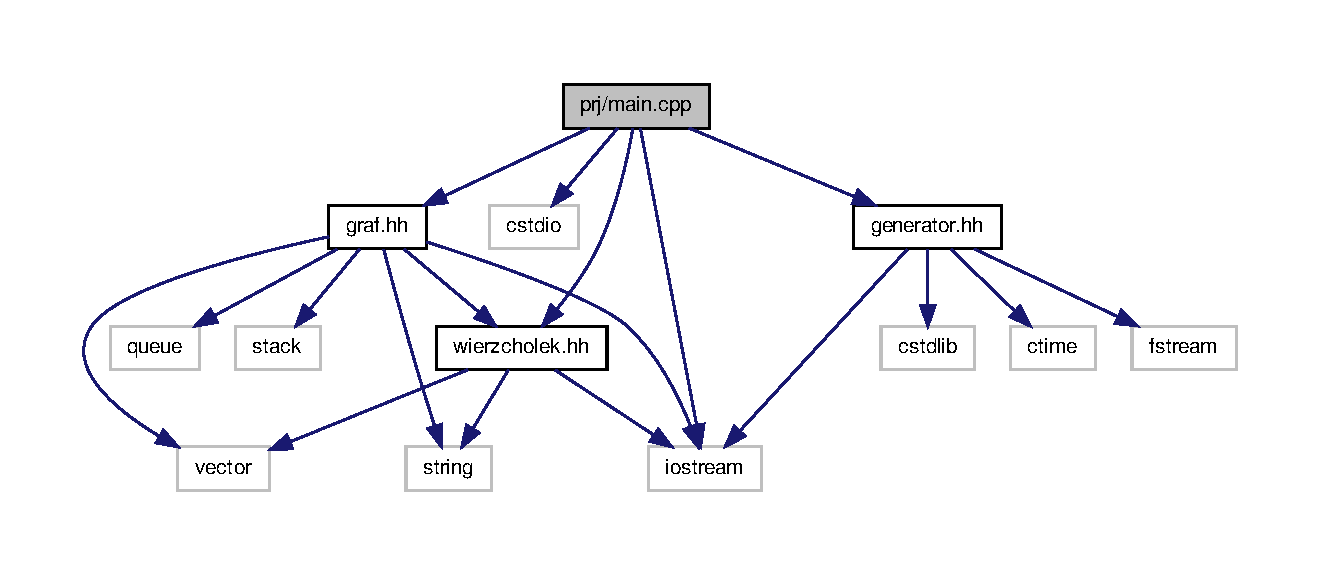
\includegraphics[width=350pt]{main_8cpp__incl}
\end{center}
\end{figure}
\subsection*{\-Defines}
\begin{DoxyCompactItemize}
\item 
\#define \hyperlink{main_8cpp_aa50aa866c5823769bb02e986d29a0589}{\-R\-O\-Z\-M\-I\-A\-R}~10000
\end{DoxyCompactItemize}
\subsection*{\-Functions}
\begin{DoxyCompactItemize}
\item 
int \hyperlink{main_8cpp_ae66f6b31b5ad750f1fe042a706a4e3d4}{main} ()
\end{DoxyCompactItemize}


\subsection{\-Define \-Documentation}
\hypertarget{main_8cpp_aa50aa866c5823769bb02e986d29a0589}{\index{main.\-cpp@{main.\-cpp}!\-R\-O\-Z\-M\-I\-A\-R@{\-R\-O\-Z\-M\-I\-A\-R}}
\index{\-R\-O\-Z\-M\-I\-A\-R@{\-R\-O\-Z\-M\-I\-A\-R}!main.cpp@{main.\-cpp}}
\subsubsection[{\-R\-O\-Z\-M\-I\-A\-R}]{\setlength{\rightskip}{0pt plus 5cm}\#define {\bf \-R\-O\-Z\-M\-I\-A\-R}~10000}}\label{main_8cpp_aa50aa866c5823769bb02e986d29a0589}


\-Definition at line 7 of file main.\-cpp.



\subsection{\-Function \-Documentation}
\hypertarget{main_8cpp_ae66f6b31b5ad750f1fe042a706a4e3d4}{\index{main.\-cpp@{main.\-cpp}!main@{main}}
\index{main@{main}!main.cpp@{main.\-cpp}}
\subsubsection[{main}]{\setlength{\rightskip}{0pt plus 5cm}int {\bf main} (
\begin{DoxyParamCaption}
{}
\end{DoxyParamCaption}
)}}\label{main_8cpp_ae66f6b31b5ad750f1fe042a706a4e3d4}


\-Definition at line 23 of file main.\-cpp.



\-Here is the call graph for this function\-:
\nopagebreak
\begin{figure}[H]
\begin{center}
\leavevmode
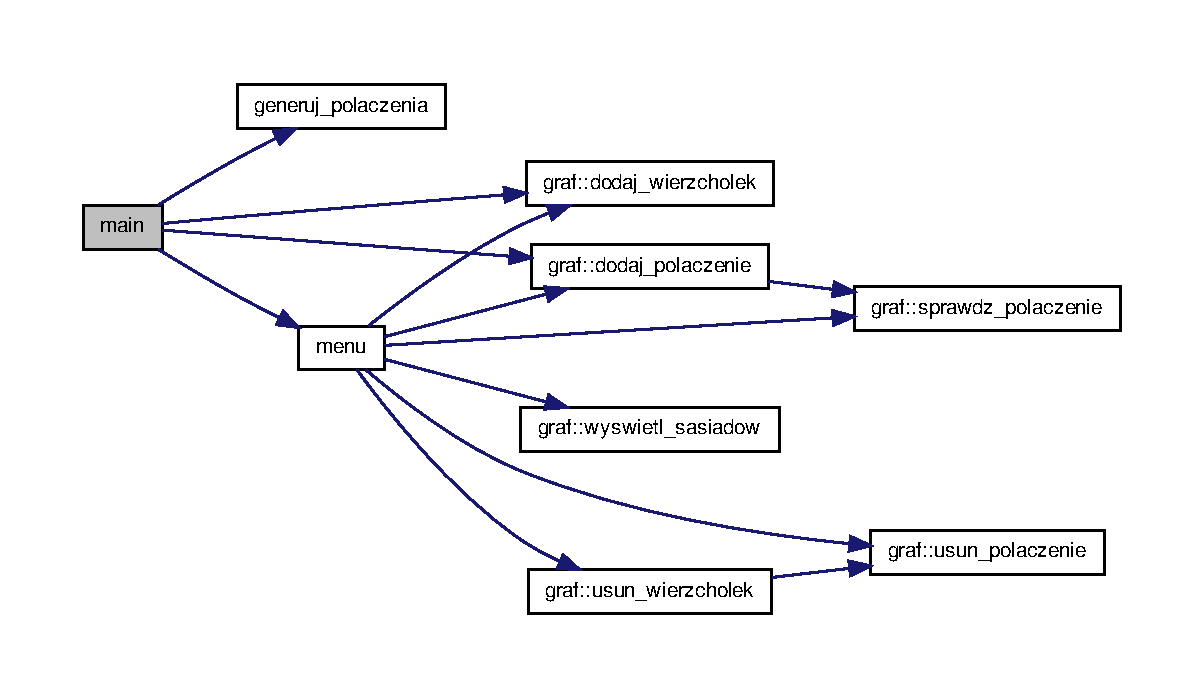
\includegraphics[width=350pt]{main_8cpp_ae66f6b31b5ad750f1fe042a706a4e3d4_cgraph}
\end{center}
\end{figure}



\hypertarget{menu_8cpp}{\section{prj/menu.cpp \-File \-Reference}
\label{menu_8cpp}\index{prj/menu.\-cpp@{prj/menu.\-cpp}}
}
{\ttfamily \#include \char`\"{}menu.\-hh\char`\"{}}\*
\-Include dependency graph for menu.\-cpp\-:
\nopagebreak
\begin{figure}[H]
\begin{center}
\leavevmode
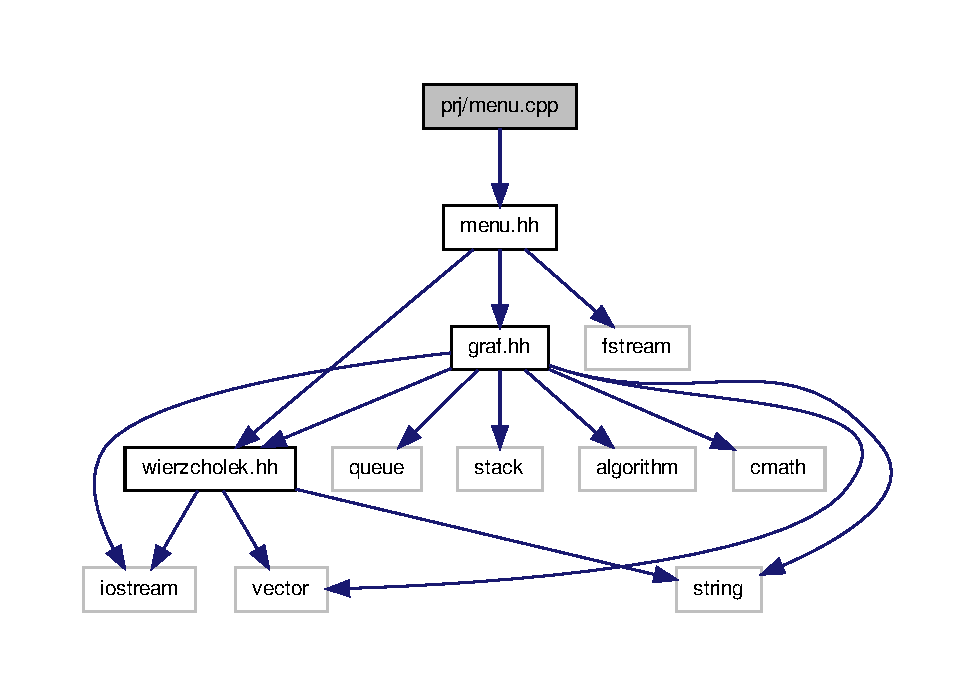
\includegraphics[width=350pt]{menu_8cpp__incl}
\end{center}
\end{figure}
\subsection*{\-Functions}
\begin{DoxyCompactItemize}
\item 
void \hyperlink{menu_8cpp_aacc433e415d518c27882997e60a20fe8}{menu} (\hyperlink{classgraf}{graf} \&graf1)
\end{DoxyCompactItemize}


\subsection{\-Function \-Documentation}
\hypertarget{menu_8cpp_aacc433e415d518c27882997e60a20fe8}{\index{menu.\-cpp@{menu.\-cpp}!menu@{menu}}
\index{menu@{menu}!menu.cpp@{menu.\-cpp}}
\subsubsection[{menu}]{\setlength{\rightskip}{0pt plus 5cm}void {\bf menu} (
\begin{DoxyParamCaption}
\item[{{\bf graf} \&}]{graf1}
\end{DoxyParamCaption}
)}}\label{menu_8cpp_aacc433e415d518c27882997e60a20fe8}


\-Definition at line 10 of file menu.\-cpp.



\-Here is the call graph for this function\-:
\nopagebreak
\begin{figure}[H]
\begin{center}
\leavevmode
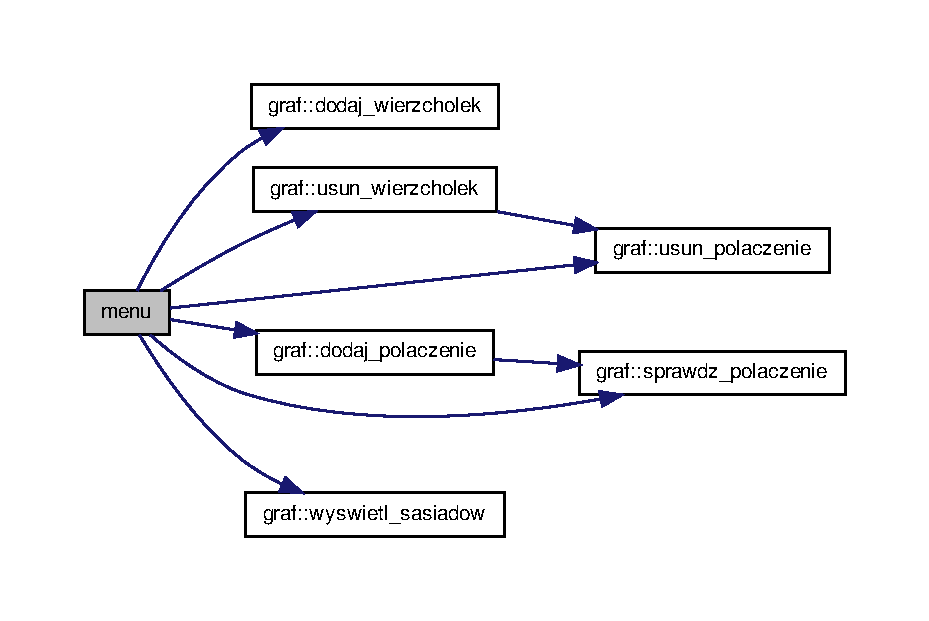
\includegraphics[width=350pt]{menu_8cpp_aacc433e415d518c27882997e60a20fe8_cgraph}
\end{center}
\end{figure}




\-Here is the caller graph for this function\-:
\nopagebreak
\begin{figure}[H]
\begin{center}
\leavevmode
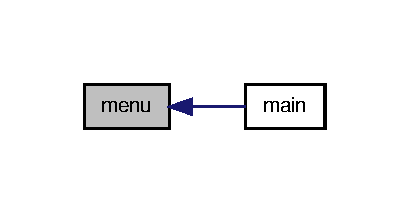
\includegraphics[width=196pt]{menu_8cpp_aacc433e415d518c27882997e60a20fe8_icgraph}
\end{center}
\end{figure}



\hypertarget{menu_8hh}{\section{prj/menu.hh \-File \-Reference}
\label{menu_8hh}\index{prj/menu.\-hh@{prj/menu.\-hh}}
}
{\ttfamily \#include \char`\"{}graf.\-hh\char`\"{}}\*
{\ttfamily \#include \char`\"{}fstream\char`\"{}}\*
{\ttfamily \#include \char`\"{}wierzcholek.\-hh\char`\"{}}\*
\-Include dependency graph for menu.\-hh\-:
\nopagebreak
\begin{figure}[H]
\begin{center}
\leavevmode
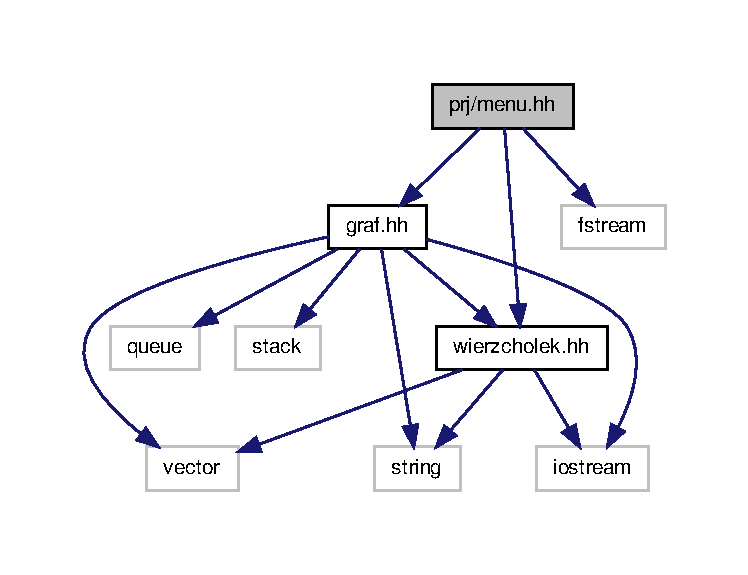
\includegraphics[width=350pt]{menu_8hh__incl}
\end{center}
\end{figure}
\-This graph shows which files directly or indirectly include this file\-:
\nopagebreak
\begin{figure}[H]
\begin{center}
\leavevmode
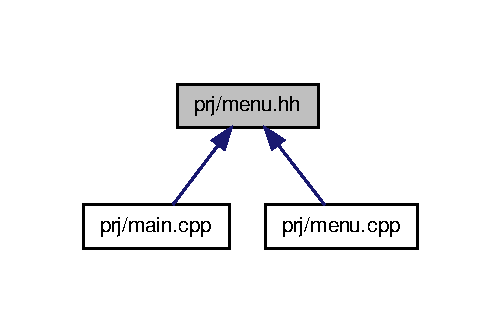
\includegraphics[width=240pt]{menu_8hh__dep__incl}
\end{center}
\end{figure}
\subsection*{\-Functions}
\begin{DoxyCompactItemize}
\item 
void \hyperlink{menu_8hh_aacc433e415d518c27882997e60a20fe8}{menu} (\hyperlink{classgraf}{graf} \&graf1)
\end{DoxyCompactItemize}


\subsection{\-Function \-Documentation}
\hypertarget{menu_8hh_aacc433e415d518c27882997e60a20fe8}{\index{menu.\-hh@{menu.\-hh}!menu@{menu}}
\index{menu@{menu}!menu.hh@{menu.\-hh}}
\subsubsection[{menu}]{\setlength{\rightskip}{0pt plus 5cm}void {\bf menu} (
\begin{DoxyParamCaption}
\item[{{\bf graf} \&}]{graf1}
\end{DoxyParamCaption}
)}}\label{menu_8hh_aacc433e415d518c27882997e60a20fe8}


\-Definition at line 10 of file menu.\-cpp.



\-Here is the call graph for this function\-:
\nopagebreak
\begin{figure}[H]
\begin{center}
\leavevmode
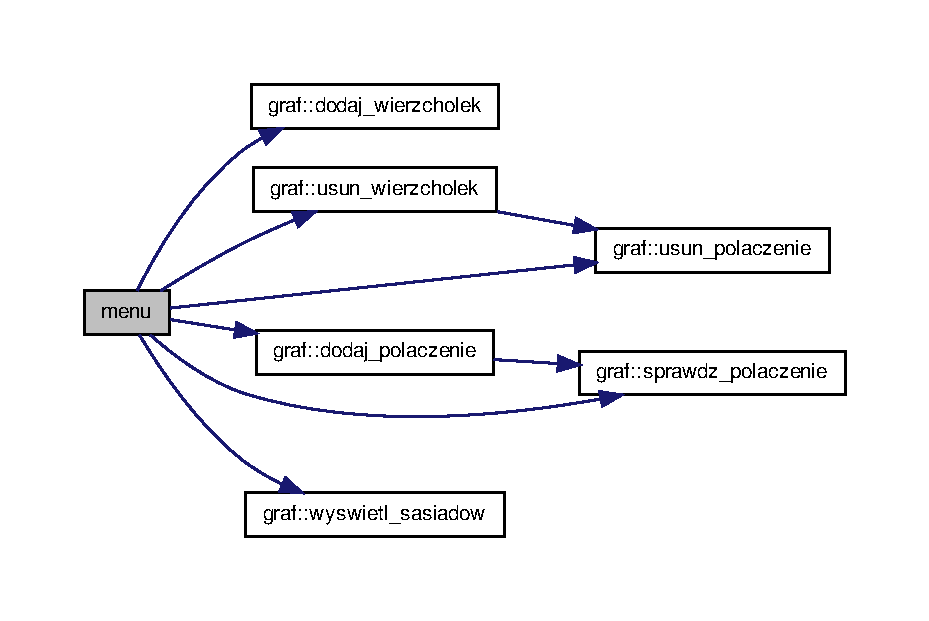
\includegraphics[width=350pt]{menu_8hh_aacc433e415d518c27882997e60a20fe8_cgraph}
\end{center}
\end{figure}




\-Here is the caller graph for this function\-:
\nopagebreak
\begin{figure}[H]
\begin{center}
\leavevmode
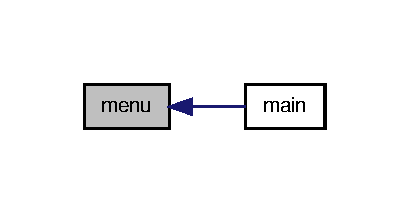
\includegraphics[width=196pt]{menu_8hh_aacc433e415d518c27882997e60a20fe8_icgraph}
\end{center}
\end{figure}



\hypertarget{stoper_8hh}{\section{prj/stoper.hh \-File \-Reference}
\label{stoper_8hh}\index{prj/stoper.\-hh@{prj/stoper.\-hh}}
}
{\ttfamily \#include $<$ctime$>$}\*
\-Include dependency graph for stoper.\-hh\-:
\nopagebreak
\begin{figure}[H]
\begin{center}
\leavevmode
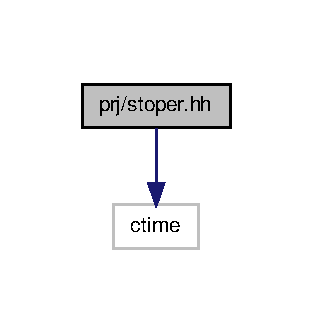
\includegraphics[width=150pt]{stoper_8hh__incl}
\end{center}
\end{figure}
\-This graph shows which files directly or indirectly include this file\-:
\nopagebreak
\begin{figure}[H]
\begin{center}
\leavevmode
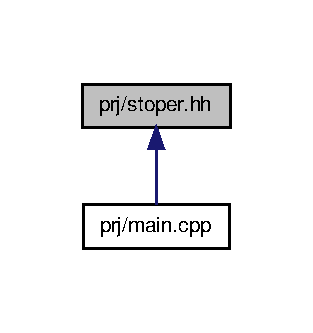
\includegraphics[width=150pt]{stoper_8hh__dep__incl}
\end{center}
\end{figure}
\subsection*{\-Classes}
\begin{DoxyCompactItemize}
\item 
class \hyperlink{classczas}{czas}
\end{DoxyCompactItemize}
\subsection*{\-Defines}
\begin{DoxyCompactItemize}
\item 
\#define \hyperlink{stoper_8hh_a3d9fc3c745d0880902fe3ea3d5d5f71e}{\-C\-L\-O\-C\-K\-S\-\_\-\-P\-E\-R\-\_\-\-S\-E\-C}~1000000
\end{DoxyCompactItemize}


\subsection{\-Define \-Documentation}
\hypertarget{stoper_8hh_a3d9fc3c745d0880902fe3ea3d5d5f71e}{\index{stoper.\-hh@{stoper.\-hh}!\-C\-L\-O\-C\-K\-S\-\_\-\-P\-E\-R\-\_\-\-S\-E\-C@{\-C\-L\-O\-C\-K\-S\-\_\-\-P\-E\-R\-\_\-\-S\-E\-C}}
\index{\-C\-L\-O\-C\-K\-S\-\_\-\-P\-E\-R\-\_\-\-S\-E\-C@{\-C\-L\-O\-C\-K\-S\-\_\-\-P\-E\-R\-\_\-\-S\-E\-C}!stoper.hh@{stoper.\-hh}}
\subsubsection[{\-C\-L\-O\-C\-K\-S\-\_\-\-P\-E\-R\-\_\-\-S\-E\-C}]{\setlength{\rightskip}{0pt plus 5cm}\#define {\bf \-C\-L\-O\-C\-K\-S\-\_\-\-P\-E\-R\-\_\-\-S\-E\-C}~1000000}}\label{stoper_8hh_a3d9fc3c745d0880902fe3ea3d5d5f71e}


\-Definition at line 11 of file stoper.\-hh.


\hypertarget{wierzcholek_8cpp}{\section{prj/wierzcholek.cpp \-File \-Reference}
\label{wierzcholek_8cpp}\index{prj/wierzcholek.\-cpp@{prj/wierzcholek.\-cpp}}
}
{\ttfamily \#include \char`\"{}wierzcholek.\-hh\char`\"{}}\*
\-Include dependency graph for wierzcholek.\-cpp\-:\nopagebreak
\begin{figure}[H]
\begin{center}
\leavevmode
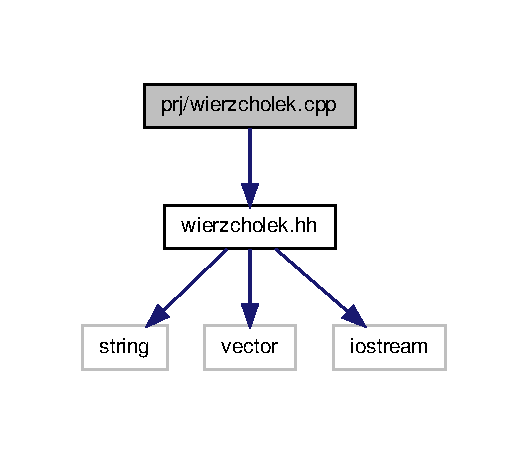
\includegraphics[width=254pt]{wierzcholek_8cpp__incl}
\end{center}
\end{figure}
\subsection*{\-Functions}
\begin{DoxyCompactItemize}
\item 
ostream \& \hyperlink{wierzcholek_8cpp_ab0941004cc1a9bb9339cf2092b1819a1}{operator$<$$<$} (ostream \&wyjscie, \hyperlink{classwierzcholek}{wierzcholek} \&wej)
\item 
istream \& \hyperlink{wierzcholek_8cpp_a221c2b565a9506a8eaed69e42e374f4e}{operator$>$$>$} (istream \&wejscie, \hyperlink{classwierzcholek}{wierzcholek} \&wyj)
\end{DoxyCompactItemize}


\subsection{\-Function \-Documentation}
\hypertarget{wierzcholek_8cpp_ab0941004cc1a9bb9339cf2092b1819a1}{\index{wierzcholek.\-cpp@{wierzcholek.\-cpp}!operator$<$$<$@{operator$<$$<$}}
\index{operator$<$$<$@{operator$<$$<$}!wierzcholek.cpp@{wierzcholek.\-cpp}}
\subsubsection[{operator$<$$<$}]{\setlength{\rightskip}{0pt plus 5cm}ostream\& operator$<$$<$ (
\begin{DoxyParamCaption}
\item[{ostream \&}]{wyjscie, }
\item[{{\bf wierzcholek} \&}]{wej}
\end{DoxyParamCaption}
)}}\label{wierzcholek_8cpp_ab0941004cc1a9bb9339cf2092b1819a1}


\-Definition at line 10 of file wierzcholek.\-cpp.

\hypertarget{wierzcholek_8cpp_a221c2b565a9506a8eaed69e42e374f4e}{\index{wierzcholek.\-cpp@{wierzcholek.\-cpp}!operator$>$$>$@{operator$>$$>$}}
\index{operator$>$$>$@{operator$>$$>$}!wierzcholek.cpp@{wierzcholek.\-cpp}}
\subsubsection[{operator$>$$>$}]{\setlength{\rightskip}{0pt plus 5cm}istream\& operator$>$$>$ (
\begin{DoxyParamCaption}
\item[{istream \&}]{wejscie, }
\item[{{\bf wierzcholek} \&}]{wyj}
\end{DoxyParamCaption}
)}}\label{wierzcholek_8cpp_a221c2b565a9506a8eaed69e42e374f4e}


\-Definition at line 21 of file wierzcholek.\-cpp.


\hypertarget{wierzcholek_8hh}{\section{prj/wierzcholek.hh \-File \-Reference}
\label{wierzcholek_8hh}\index{prj/wierzcholek.\-hh@{prj/wierzcholek.\-hh}}
}
{\ttfamily \#include $<$string$>$}\*
{\ttfamily \#include $<$vector$>$}\*
{\ttfamily \#include $<$iostream$>$}\*
\-Include dependency graph for wierzcholek.\-hh\-:\nopagebreak
\begin{figure}[H]
\begin{center}
\leavevmode
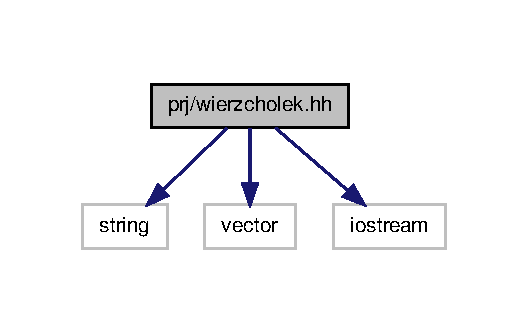
\includegraphics[width=254pt]{wierzcholek_8hh__incl}
\end{center}
\end{figure}
\-This graph shows which files directly or indirectly include this file\-:\nopagebreak
\begin{figure}[H]
\begin{center}
\leavevmode
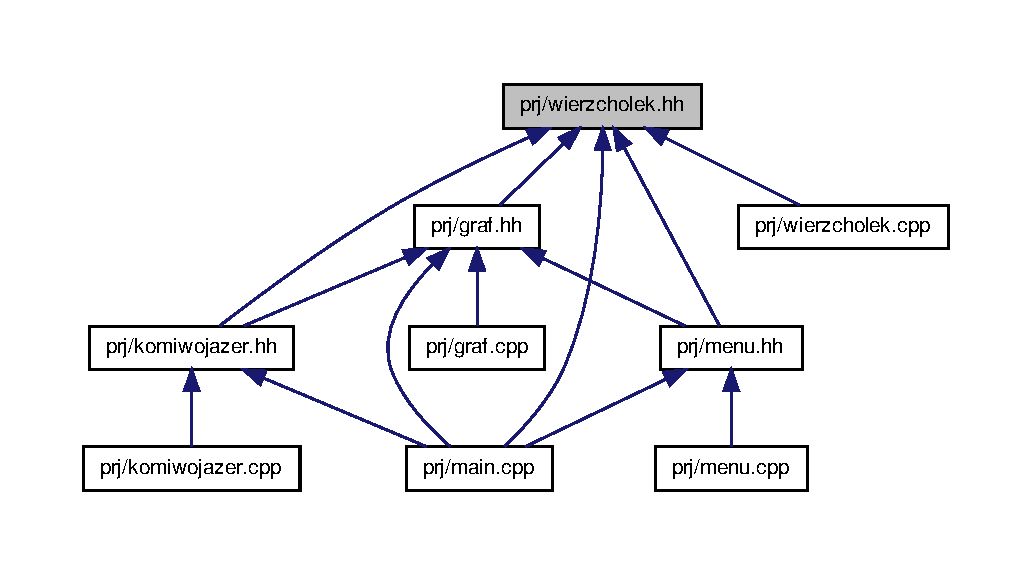
\includegraphics[width=350pt]{wierzcholek_8hh__dep__incl}
\end{center}
\end{figure}
\subsection*{\-Classes}
\begin{DoxyCompactItemize}
\item 
struct \hyperlink{structpolaczenie}{polaczenie}
\begin{DoxyCompactList}\small\item\em clasa modeluje pojecie pojecie poedynczego wierzcholka grafu \end{DoxyCompactList}\item 
class \hyperlink{classwierzcholek}{wierzcholek}
\item 
struct \hyperlink{structelement__bfs}{element\-\_\-bfs}
\begin{DoxyCompactList}\small\item\em struktura definiuje element drzewa przechodzenie w szerz \end{DoxyCompactList}\item 
struct \hyperlink{structelement__dfs}{element\-\_\-dfs}
\begin{DoxyCompactList}\small\item\em element drzewa przejscia dla przeszukiwania w głąb; \end{DoxyCompactList}\item 
struct \hyperlink{structelement__a}{element\-\_\-a}
\end{DoxyCompactItemize}
\subsection*{\-Functions}
\begin{DoxyCompactItemize}
\item 
bool \hyperlink{wierzcholek_8hh_abf7cee761b1201166cbe397d8723789a}{porownanie} (\hyperlink{structpolaczenie}{polaczenie} aaa, \hyperlink{structpolaczenie}{polaczenie} bbb)
\end{DoxyCompactItemize}


\subsection{\-Function \-Documentation}
\hypertarget{wierzcholek_8hh_abf7cee761b1201166cbe397d8723789a}{\index{wierzcholek.\-hh@{wierzcholek.\-hh}!porownanie@{porownanie}}
\index{porownanie@{porownanie}!wierzcholek.hh@{wierzcholek.\-hh}}
\subsubsection[{porownanie}]{\setlength{\rightskip}{0pt plus 5cm}bool {\bf porownanie} (
\begin{DoxyParamCaption}
\item[{{\bf polaczenie}}]{aaa, }
\item[{{\bf polaczenie}}]{bbb}
\end{DoxyParamCaption}
)}}\label{wierzcholek_8hh_abf7cee761b1201166cbe397d8723789a}


\-Definition at line 9 of file wierzcholek.\-cpp.



\-Here is the caller graph for this function\-:
\nopagebreak
\begin{figure}[H]
\begin{center}
\leavevmode
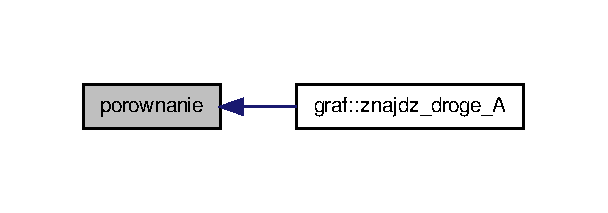
\includegraphics[width=292pt]{wierzcholek_8hh_abf7cee761b1201166cbe397d8723789a_icgraph}
\end{center}
\end{figure}



\printindex
\end{document}
